\chapter{Visual Exploration of Human-Scale Urban Forms Based on Street Views}\label{chap:intro}
\QM{Urban forms at human-scale, i.e., urban environments that individuals can sense (e.g., sight, smell, and touch) in their daily lives, can provide unprecedented insights on a variety of applications, such as urban planning and environment auditing.
The analysis of urban forms can help planners develop high-quality urban spaces through evidence-based design.
However, such analysis is complex because of the involvement of spatial, multi-scale (i.e., city, region, and street), and multivariate (e.g., greenery and sky ratios) natures of urban forms.
In addition, current methods either lack quantitative measurements or are limited to a small area. 
The primary contribution of this work is the design of StreetVizor, an interactive visual analytics system that helps planners leverage their domain knowledge in exploring human-scale urban forms based on street view images.
Our system presents two-stage visual exploration: 
1) an AOI Explorer for the visual comparison of spatial distributions and quantitative measurements in two areas-of-interest (AOIs) at city- and region-scales;
2) and a Street Explorer with a novel parallel coordinate plot for the exploration of the fine-grained details of the urban forms at the street-scale.
We integrate visualization techniques with machine learning models to facilitate the detection of street view patterns. 
We illustrate the applicability of our approach with case studies on the real-world datasets of four cities, i.e., Hong Kong, Singapore, Greater London and New York City.
Interviews with domain experts demonstrate the effectiveness of our system in facilitating various analytical tasks.}

\section{Introduction}
%%%%%%%%%%%%%%%%%%%%%%%%%%%%%%%%%%%%%%%%%%%%%%%%%%%%%%%%%%%%%%%%%%%%%%%%
Human-scale urban form describes fine-scale characteristics of urban environments that can be directly seen, touched, and experienced by a city's residents in their daily lives~\cite{long_2016_human-scale}.
It is typically measured in high-resolution by sight and hearing, i.e., from several to tens of meters.
Compared with a city's scale, which is usually measured in kilometers, this scale is human-oriented.
 % and allows people to interact with surrounding environments.
% For instance, views on two neighboring streets can be totally different, even though the streets are very close to each other.
As humans pay more attention to interactive surroundings~\cite{gehl_1971_life}, understanding human-scale urban forms is essential for urban planners in designing high-quality urban spaces. 
However, traditional urbanism theories, such as small-scale surveys and mapping, are hard to provide in-depth guidance for effective urban planning and design at this fine scale.

Given the advancement of various sensing technologies, e.g., cameras and GPS devices, we can now quantitatively measure human-scale urban forms by analyzing big urban data.
In particular, services, such as Google Street View (GSV)~\cite{anguelov2010google}, provide detailed panoramic views of urban space from different geographic positions
These panoramic views can be utilized to measure various features, including greenery coverage and sky visibility, of human-scale urban forms visible to human eyes.
Some pioneering studies have shown that neighborhood environment~\cite{rundle_2011_using}, street-level greenery~\cite{li_2015_accessing}, and even street safety~\cite{Naik_2014_streetscore} can be precisely assessed from these views.
 % through analyzing GSV images.

However, GSV image exploration mainly focuses on either a particular feature (e.g., greenery coverage~\cite{li_2015_accessing}) or a small area (e.g., neighborhood~\cite{rundle_2011_using} and street~\cite{Naik_2014_streetscore, li_2015_accessing}).
This deficiency limits its applicability in urban planning, where planners need to 
1) quantitatively measure multivariate features of urban forms, including not only greenery coverage, but also sky visibility, and vehicle density~\cite{long_2017_how}; 
2) systematically explore urban forms in areas-of-interest (AOIs) at multiple scales, i.e., from small (e.g., streets) to mid (e.g., districts) to large scales (e.g., cities)~\cite{liu_2015_understanding}.
In addition, direct means for the comparison of urban forms in two AOIs is desirable to allow planners to utilize information for the quick identification and improvement of factors that affect the quality of urban space.

A visual analytics tool is necessary to fulfill these requirements because it can integrate powerful computing capabilities to quantitatively measure multivariate features, with interactive visual interfaces to systematically explore and compare features in AOIs on demand~\cite{sun_2013_survey}.
Developing such a tool requires considerable effort because of the following reasons:
first, as cities comprise vast amounts of street views, an efficient feature extraction algorithm is required to automatically uncover human-scale urban forms.
Second, the development of a tool for the visual comparison of multivariate features in two AOIs requires an effective visual design that tackles the challenges of spatial, multivariate, and comparative data visualizations.

In this paper, we introduce StreetVizor, a visual analytics system for the exploration of human-scale urban forms based on GSV images.
We develop the system in an iterative design process: specific analysis requirements are described by a collaborating urban planner, and the designs are evaluated and refined against requirements.  
To present information in concisely, StreetVizor combines a set of well-established visualization techniques, including coordinated multiple views (CMVs) and scatterplot matrix, with a new design of parallel coordinates that integrate street layout information.
Our system utilizes advanced clustering models to enable the efficient exploration of street view patterns.
We apply StreetVizor in real-world datasets containing $\sim$1.7 million of GSV images of four cities: Singapore, Hong Kong, Greater London, and New York City, and demonstrate its effectiveness through interviews with domain experts. 

\vspace*{2mm}
The main contributions of this work include:

\begin{itemize}
	
\vspace*{-1.5mm}
\item
A fully automatic approach measuring human-scale urban forms by applying deep learning techniques on GSV images;
	
\vspace*{-1.5mm}
\item
A visual comparison framework for exploring human-scale urban forms on city-, region-, and street-scales;
	
\vspace*{-1.5mm}
\item
A novel visual design of parallel coordinates that integrate street layout information;
	
\vspace*{-1.5mm}
\item
Interesting insights revealed from case studies and expert interviews, such as the negative correlation between $greenery$ and $building$ features, and the differences in street views of two cities.
		
\end{itemize}
% \vspace*{-1mm}
\section{Related Work}
\label{sec:c1_related_work}

This section discusses previous studies closely related to our work.

%===============================================
\subsection{Street View Analysis}
GSV system provides high quality and accurate panoramic images of hundreds of cities~\cite{anguelov2010google}.
In recent years, researchers studying human-scale urban forms have utilized GSV images as a new and convenient data source. 
For example, researches have shown that the analysis of GSV images can be used to audit neighborhood environments~\cite{rundle_2011_using}, quantify street greenery~\cite{li_2015_accessing}, and predict street safety~\cite{Naik_2014_streetscore}.
Nonetheless, the majority of these studies face scalability issues given their focus on either a particular feature~\cite{li_2015_accessing} or a small area~\cite{rundle_2011_using, Naik_2014_streetscore, li_2015_accessing}.
Thees issues can be addressed by incorporating deep learning techniques, which can be used to summarize city landscapes~\cite{doersch2015makes} and estimate the demographic makeup of a country~\cite{gebru2017using}.

In this work, we collect $\sim$1.7 million GSV images of four representative mega-cities, and apply a deep learning technique~\cite{Badrinarayanan_2015_segnet} to automatically extract desired urban forms from the collected images.
More importantly, we develop an effective visual analytics tool for urban planners to explore human-scale urban forms.

%===============================================
\subsection{Urban Data Visualization}
Vast amounts of urban data, including traffic~\cite{ferreira_visual_2013, wang_2013_visual}, social media~\cite{xu_2013_visual, chen_2015_interactive}, environment~\cite{ferreira_2011_birdvis}, and simulated urban spaces~\cite{vanegas_2009_visualization}, have been collected in an urban context.
Big urban data brings in unprecedented opportunities for evidence-based urban design, and visualization systems can assist domain experts in finding evidence from the data.
A systematic overview of visualization systems can be found in~\cite{zheng_2016_visual}.

Qu et al.~\cite{qu_2007_visual} presented a comprehensive visualization system for the analysis of a city's air pollution that affects the daily lives of residents.
Their system integrates parallel coordinates and scatterplots to show relationships between high-dimensional air pollutants.
In addition to air pollution, landmark visibility is related to the daily experience of a city's residents.
Ortner et al.~\cite{ortner_2016_vis-a-ware} visually compared the effects of candidate buildings on landmark visibility from various viewpoints.
In this system, users can select a series of ranking schemes, and candidate buildings are then automatically sorted.
Similar to our present work, Arietta et al.~\cite{arietta_2014_city} associated visual elements with city attributes, including violent crime rates and housing prices.
They developed various prototype visualizations, such as the visual boundary of urban neighborhoods.

% \vspace{2mm}
Although different data are explored, these visualizations similarly employ CMVs, because urban data typically exhibits both spatial information and multi-dimensional attributes.
Our system also adopts this empirical approach.
In addition, to address specific domain problems, we develop effective visualization techniques, including a novel parallel coordinates enhanced with street layouts.

%===============================================
\subsection{Multivariate Geographical Data Visualization}
Visualizing multivariate data is a hot topic in the visualization field.
Numerous conventional approaches to this topic have been developed, and can be classified into two groups:
1) employing visualization techniques, such as parallel coordinates plot (PCP), scatterplot matrix, and start coordinates;
and 2) projecting data points onto a two- or three-dimensional visual space that can be directly plotted on a screen, such as multidimensional scaling and principal component analysis.
All these approaches have pros and cons.
For example, although PCP presents all dimensional attributes without information loss, it can easily generate visual clutter with big data and pairwise correlations can only be shown on two nearby coordinates~\cite{heinrich_2012_state}.
Many improvements have been developed to address these issues.
These improvements include edge bundling to reduce visual clutter~\cite{zhou2008visual, holten_2010_evaluation}, and hierarchical data clustering and the navigation of resulting structures~\cite{fua1999hierarchical, zhao_2012_structure}.
% ., and sort dimensions in order based on their correlations~\cite{zhao_2012_structure, wu_2015_telcovis}.

When multivariate data is dependent upon locations, the analytical tasks become more complex because geographical information needs to be revealed.
Turkay et al. developed \textit{Attribute Signature}~\cite{turkay_2014_attribute}, which employs a geographical map and small multiples of multivariate attributes to show geographic variability in attribute statistics.
Goodwin et al.~\cite{goodwin_2016_visualizing} further explored multivariate geographical data across scales by adopting new designs to show correlation, scale, and geographical information.
The frameworks proposed by both studies can be generalized to explore multivariate geographical data.

In this work, human-scale urban forms to be explored are also multivariate geographical data: the features are in six dimensions and they are dependent on locations.
We leverage the advantages of scatterplot matrix and PCP for different analytical tasks.
Specifically, we employ scatterplot matrix for exploring features at city- and region scales given that it can effectively reveal correlations between all pair-wise features.
We also arrange the views in a way similar to \textit{Attribute Signature}~\cite{turkay_2014_attribute}, i.e., geographical information is presented on maps and multivariate attributes in small multiples. 
In addition, we develop a novel PCP enhanced with a themeriver plot, which fits better with the analytical task of showing feature variations along street layout at street-scale.

%===============================================
\subsection{Comparative Visualization}
Gleicher et al.~\cite{gleicher_2011_visual} classified techniques for visual comparison into three categories:
1) Juxtaposition, i.e., presenting objects next to each other. 
For example, NodeTrix~\cite{yang_2017_blockwise} arranges two human brain networks side-by-side. 
2) Superposition, i.e., presenting multiple objects on top of one another.
Typical examples are time-series line graphs that plot the changes in several variables over time in the same coordinate system.
3) Explicit encoding, i.e., presenting differences or correlations between objects visually.
For instance, the bivariate density map is employed in~\cite{zeng_2017_visualizing} to show the relationship between departure and arrival movements over space.
In practice, these techniques are combined to address complex analytical tasks.

Our work adopts juxtaposition that arranges maps of two AOIs/streets side-by-side (Fig.~\ref{fig:c1_teaser}(b) \& (d)), and superposition to compare multivariate features of two AOIs/streets in the same coordinate system (Fig.~\ref{fig:c1_teaser}(c) \& (e)).

\if 0
\subsection{Human-scale Urban Form}
Though human-scale urban form is defined recently~\cite{long_2016_human-scale}, discussions of the concept in urban planning and designing have a long history that can be traced to 1960s.
A series of pioneering studies~\cite{jacobs_1961_life, gehl_1971_life} claimed the positive effects of human-scale urban form in designing high-quality urban space.
Among various types of human-scale urban form, the visible one is particularly important as human beings tend to pay most attentions to surroundings that can be directly seen~\cite{gehl_1971_life}. 

Accompanying with the raising of big open data, e.g., GSV images, researches in studying visible human-scale urban form are focusing on quantitatively measuring the related features nowadays. 
For example, researches have shown that analyzing GSV images can audit neighborhood environments~\cite{rundle_2011_using}, quantify street greenery~\cite{li_2015_accessing} and predict street safety~\cite{Naik_2014_streetscore}.
Nonetheless, most of these researches got scalability issues as they focused on either a particular feature or a small area.
The issues can be addressed by incorporating deep learning techniques, by which recent studies have shown its applicability in summarizing landscape of a city~\cite{doersch2015makes} and even estimating demographic makeup of a country~\cite{gebru2017using}.

\vspace{2mm}
In this work, we first identify the important features of visible human-scale urban form, then collect millions of GSV images across four representative mega-cities, and apply a deep learning technique - SegNet~\cite{Badrinarayanan_2015_segnet} - to automatically label related features in the images.
More importantly, we develop an effective visual analytical tool for urban planners to explore the analysis on demand.

\fi

\if 0
\subsection{Street view images analysis}

Google street view(GSV) is a well know system that provides panoramic images in hundreds of cities of more than 20 countries to millions of googles users. During the past 15 year, GSV system can provide a good quality and accurate images service, and more and more researchers begin to focus on this data source\cite{anguelov2010google}. GSV is considered as a novel and convenient way to collect environmental information and has been utilized in a broad range of research domains including ecology, geography, archeology, urbanology and even some social science. 

In recent years, the researchers in the ecology field found that the GSV images was an alternative way to observe the natural environment. Olea et al. \cite{olea2013assessing} discussed that the GSV images could be a good data source to assess the habit of some cliff living animals and the using of both of these two methods could be highly useful as a coarse-scale assessment method over large geographic areas. Hardion et al.\cite{hardion2016species} proposed a  time and cost-effective solution using the geo-located street view images in the analysis of species distributions. In the discipline of urbanology and sociology, GSV has been used in the virtual audit of different physical environment\cite{clarke2010using, rundle2011using, kelly2013using, vanwolleghem2014assessing} in the city. These methods has the potential to significantly reduce the costs and time of collecting data and can be well adapted in the large geo-scale research. 

Even though the GSV images could be adapted in different research areas, in the most instance, the observation of environment is still conducted by human beings. Nowadays, fast developed of deep learning techniques has been widely used in image processing, many research has considered the automatic methods to further reduce the human cost. Doersch et al.\cite{doersch2015makes} analyzed millions of image from GSV to extract the visual features commonly occurred to summary the landscape of a city. Timnit et al.\cite{gebru2017using} also proposed a method use deep learning techniques and GSV images to estimate teh demographic makeup of United States.
\fi

\section{Background and Analytical Tasks}
In this section, we introduce our research background and summarize the desired analytical tasks.

\subsection{Background}
\label{sec:bg}

Although the concept of human-scale urban form has only been recently defined~\cite{long_2016_human-scale}, its discussions in the context of urban planning has a long history that can be traced back to the 1960s.
A series of pioneering studies~\cite{jacobs_1961_life, gehl_1971_life} claimed the positive effects of understanding human-scale urban forms in designing high-quality urban space.
Visible human-scale urban forms are particularly important as human beings tend to pay most attentions to surroundings that can be directly seen~\cite{gehl_1971_life}. 

Over the past 10 months, we closely worked with a senior researcher ($SR$) in the field of evidence-based urban design $-$ an emerging research topic in urban planning and design.
$SR$ pointed out that though urban planners have begun to realize the importance and usefulness of street views in analyzing visible urban forms (e.g.,~\cite{rundle_2011_using, li_2015_accessing, Naik_2014_streetscore}), systematic and efficient methods that can facilitate exploration remain lacking.
Hence, $SR$ proposed the development of an efficient visual analytics tool for exploring human-scale urban forms based on GSV images.

To better understand the problem domain, we conducted several rounds of structured interviews with $SR$.
The main analysis criteria are summarized below:

\vspace*{-2mm}
\begin{itemize}

\item
\textbf{Multivariate Features.}
As images contain rich information on the urban environment, the first step is to identify the urban forms for analysis.
Here, we identify five key features that can reflect the quality and livability of street spaces~\cite{jacobs_1961_life, gehl_1971_life}, i.e., $greenery$, $sky$, $building$, $road$, and $vehicle$ features.
$Greenery$ reflects the pleasing greenery view of a street; 
$sky$ and $building$ are correlated with the sense of street closure negatively and positively, respectively; 
and increments in $road$ and $vehicle$ ratios decrease the willingness of people to walk and street attractiveness.

\vspace*{-1mm}
\item
\textbf{Street View Crawling.}
To reveal the surrounding scenes of a street space, street views have to be crawled appropriately: successive images should reflect the continuous change in surrounding scenes.
Hence, the distance between two successive views should not exceed a limit that produces discontinuous scenes; meanwhile, it should not be too small, which will cause computing overload. 
After experimenting with several options, we find 50 meters is a suitable value for the distance between two successive views.

\vspace*{-1mm}
\item
\textbf{Street View Directions.}
Although GSV~\cite{gsv_api} provides 360-degree panorama imagery, only the front and back images in the directions of street headings at sampling locations are required. 
Side views are not utilized because of the following considerations: 
First, side views mainly present building facades and street sides and thus cannot correctly reflect other key features of street space, e.g., $road$.
Second, side views are partially contained by the front and back images at nearby sampling locations. 

\end{itemize}

\vspace*{-1mm}
To evaluate the effectiveness of our approach, we first experiment with a few representative cities.
$SR$ suggested Hong Kong, Singapore, Greater London, and New York City:
Hong Kong and Singapore are dense cities with high-rise buildings in Asia.
Greater London and New York City are well-planned cities in Europe and the US.

%===============================================
\subsection{Analytical Tasks}
\label{ssec:tasks}

After identifying the analysis criteria, $SR$ further raised a list of questions for our system to address, including:
\textit{How are the identified features distributed in an AOI?
What are the feature differences between two AOIs?
What are the exact views that people can see on a street?
Are there any representative views?}

Based on these questions, we compile a list of analytical tasks:

\vspace*{-2mm}
% \begin{enumerate}[label={T.\arabic*:}]
\begin{itemize}

\item \textbf{\QM{T1. Efficient Multi-scale Exploration:}}
Human-scale urban forms are associated with street views at different locations that can be organized on city-, region- and street-scales.
Planners first need an intuitive overview of the identified feature distributions within a city or a region (T.1.1).
Next, planners need to explore the details of the urban forms, such as the exact street views, at street level (T.1.2).
Effective interactions are required to assist users in navigating across different scales.

\vspace*{-1.5mm}
\item \textbf{T2. Quantitative Measurements:}
% Traditionally, planners usually evaluate a street space qualitatively based on their preferences and experiences on the street views.
% This can easily lead to inconsistent evaluation due to the differences among planners.
$SR$ emphasized the importance of quantitative measurements to evidence-based urban design.
Here, given that an AOI/street can contain vast amounts of street views, planners should analyze the statistics of identified features, including correlations between features, distributions, and standard deviations (T.2.1).
Filtering street views against the values of a specific feature is also important (T.2.2).

\vspace*{-1.5mm}
\item \textbf{T3. Effective Ranking and Comparison:}
% The capability to compare human-scale urban forms in two AOIs/streets is important, as planners can leverage their domain knowledge to gain deep insights into factors affecting the quality of street space.
To help planners quickly narrow down the exploration scope, features among multiple AOIs/streets should be effectively ranked (T.3.1).
Areas/streets with certain features of high values can be easily discovered for further exploration.
After planners select two AOIs/streets, they need to compare the differences in spatial distributions (T.3.2) and the quantitative measurements (T.3.3) of the urban forms. 
% \qm{In addition, effective ranking methods(T.3.3) for the multi features is also helpful for the planers to explore multiple AOIs/streets and narrow down the research scope.}  

\end{itemize}
\section{System Framework}



%===============================================
\begin{figure}[t]
	\centering
	% \vspace{-4mm}
	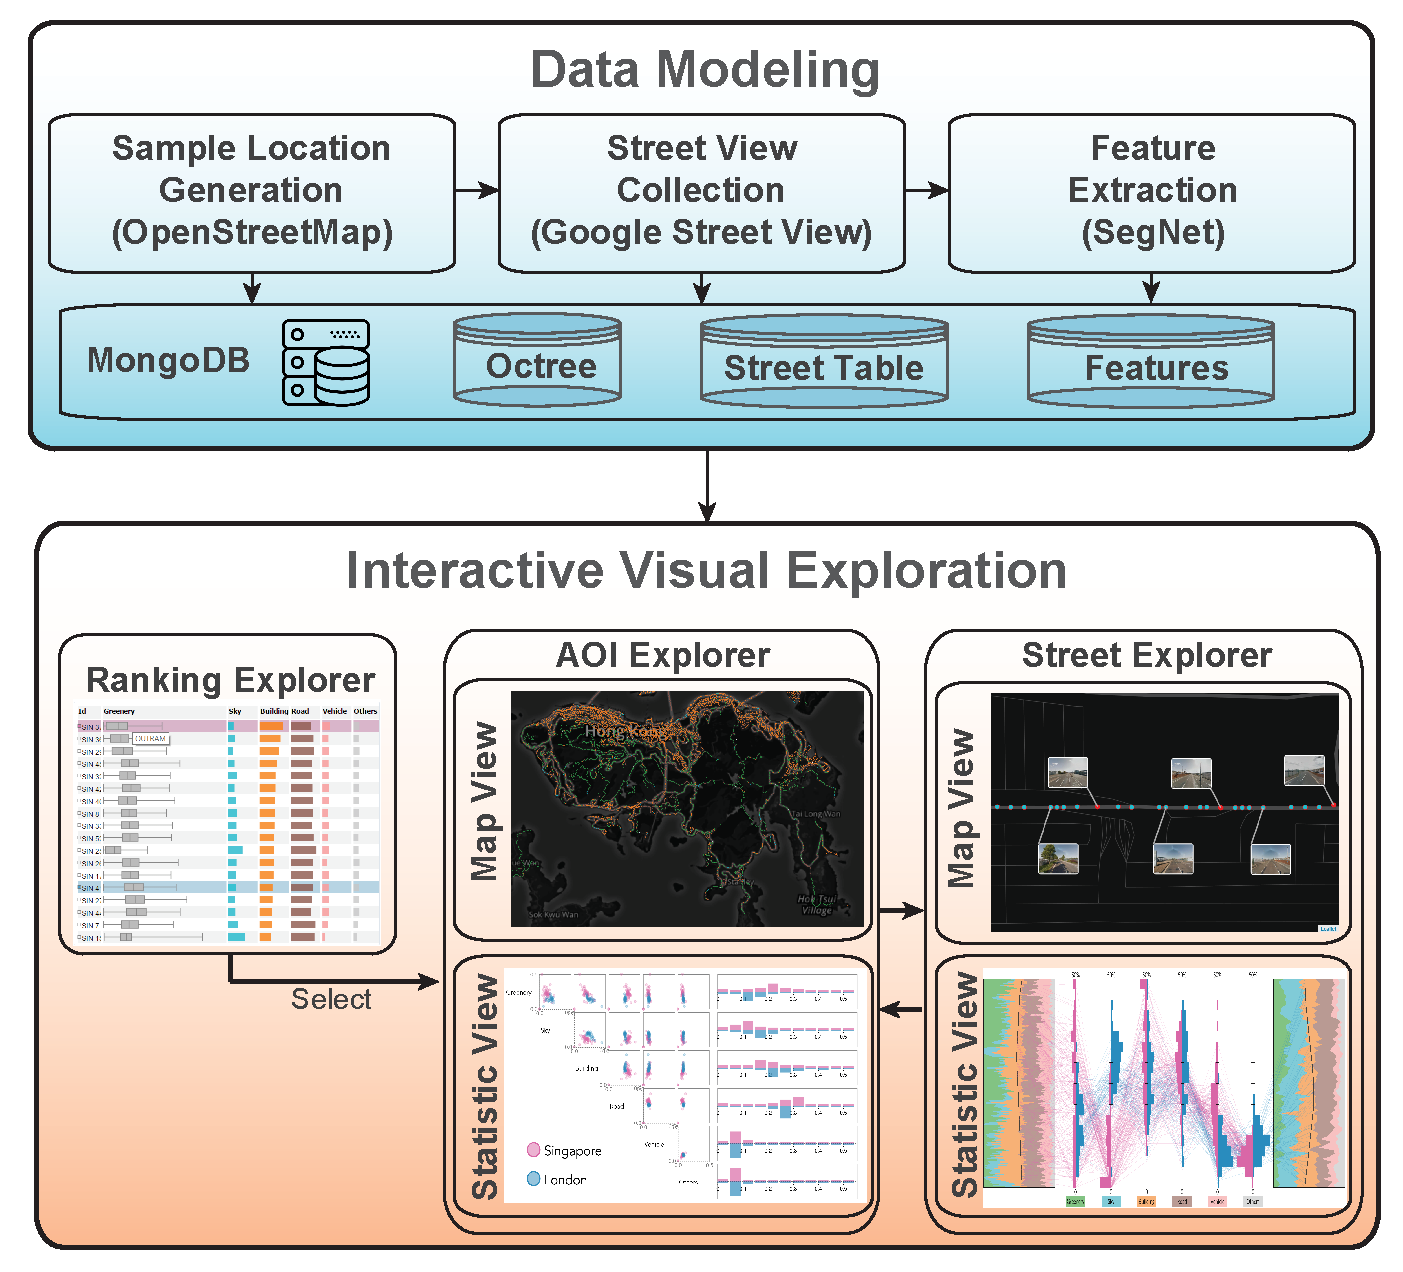
\includegraphics[width=0.9\columnwidth]{figure/streetvizor/fig2_framework/framework}
	\vspace{-5mm}
	\caption{Overview of StreetVizor workflow. Our system consists of two phases: data modeling and interactive visual exploration.}
	\label{fig:c1_sys_overview}
	\vspace{-6mm}
\end{figure}

StreetVizor is a web-based application comprising two major phases, as illustrated in Fig.~\ref{fig:c1_sys_overview}.
In the data modeling phase, our system automatically collects hundreds of thousands of GSV images at sampling positions in each city generated from OpenStreetMap (OSM) (Section~\ref{ssec:c1_data_collection}).
Then, we classify the pixels of the collected images into 12 classes using SegNet, and extract the desired feature metric from the classification results (Section~\ref{ssec:c1_feature}).
Data collection and preprocessing are conducted offline on a high-performance workstation with 12 core 3.40 GHz Intel Core i7-6800K CPU and a GeForce GTX 1080 graphics card.
Though enabled with GPU acceleration, the computation still takes several to 20 hours to preprocess images from each city.
Then, we construct data structures, including an octree and a lookup table, to facilitate visual exploration, such as spatial query and filtering (Section~\ref{ssec:c1_query}).
The datasets are stored in a back-end MongoDB server with 2.4 GHz Intel Xeon E5-2620 CPU and 64 GB memory.

The interactive visual exploration phase consists of two stages:
1) Our system provides users with a Ranking Explorer that ranks and compares multiple AOIs/streets based on human-scale urban forms.
Users can narrow down exploration by selecting two AOIs/streets for detailed comparison. 
2) If two AOIs are selected, the system will present an AOI Explorer that compares the differences in human-scale urban forms in two AOIs at city- and region-scales.
The AOI Explorer is composed of CMVs, including two juxtaposition map views for spatial exploration and a superposition statistic view for comparing various quantitative measurements, such as feature correlations and diversities.
Users can further navigate down to select two streets, and our system will provide Street Explorer, which presents the fine details of human-scale urban forms at street-level.
In Street Explorer, we present map views that show the geographical information and representative images of two streets.
We also develop a novel PCP enhanced with themeriver along street layouts, allowing users to compare multivariate features and reveal feature distributions along the two streets.
The visualization modules are implemented in D3.js and Three.js for different rendering requirements, and they are integrated using Vue.js.

\if 0

. Whole system framework is shown in the figure.2.
The whole system pipeline starts from the data process models. Data process model will collect and analysis Google street view images, mark them with gps tags and generate the human-scale feature vector automatically . The output of the human-scale features with gps information will be stored by mongodb, a nosql database, the correponding geographical index will be generated to improve query speed. Based on mongodb, we build web server with Python/Flask, and Frontend system with Vuejs. The viusalization module are implemented by D3 and Three.js for different render requirement.

The visualization module consists of tow major view: navigation view and analysis view. Navigation view provides high level overview of the human-scale feature distribution as well as many flexible query methods. Users can navigate from different level in the navigation view, to find the analysis target or narrow down to a smaller scope, e.g. a smaller subset of streets or regions. For the selected units, users can conduct an find granularity analysis...

\fi
\section{Data Modeling}
In this section, we first describe the collection of GSV images and the extraction of human-scale urban forms from the collected images.
Furthermore, we present the methods for data querying and filtering.

\begin{figure}[t]
	\centering
	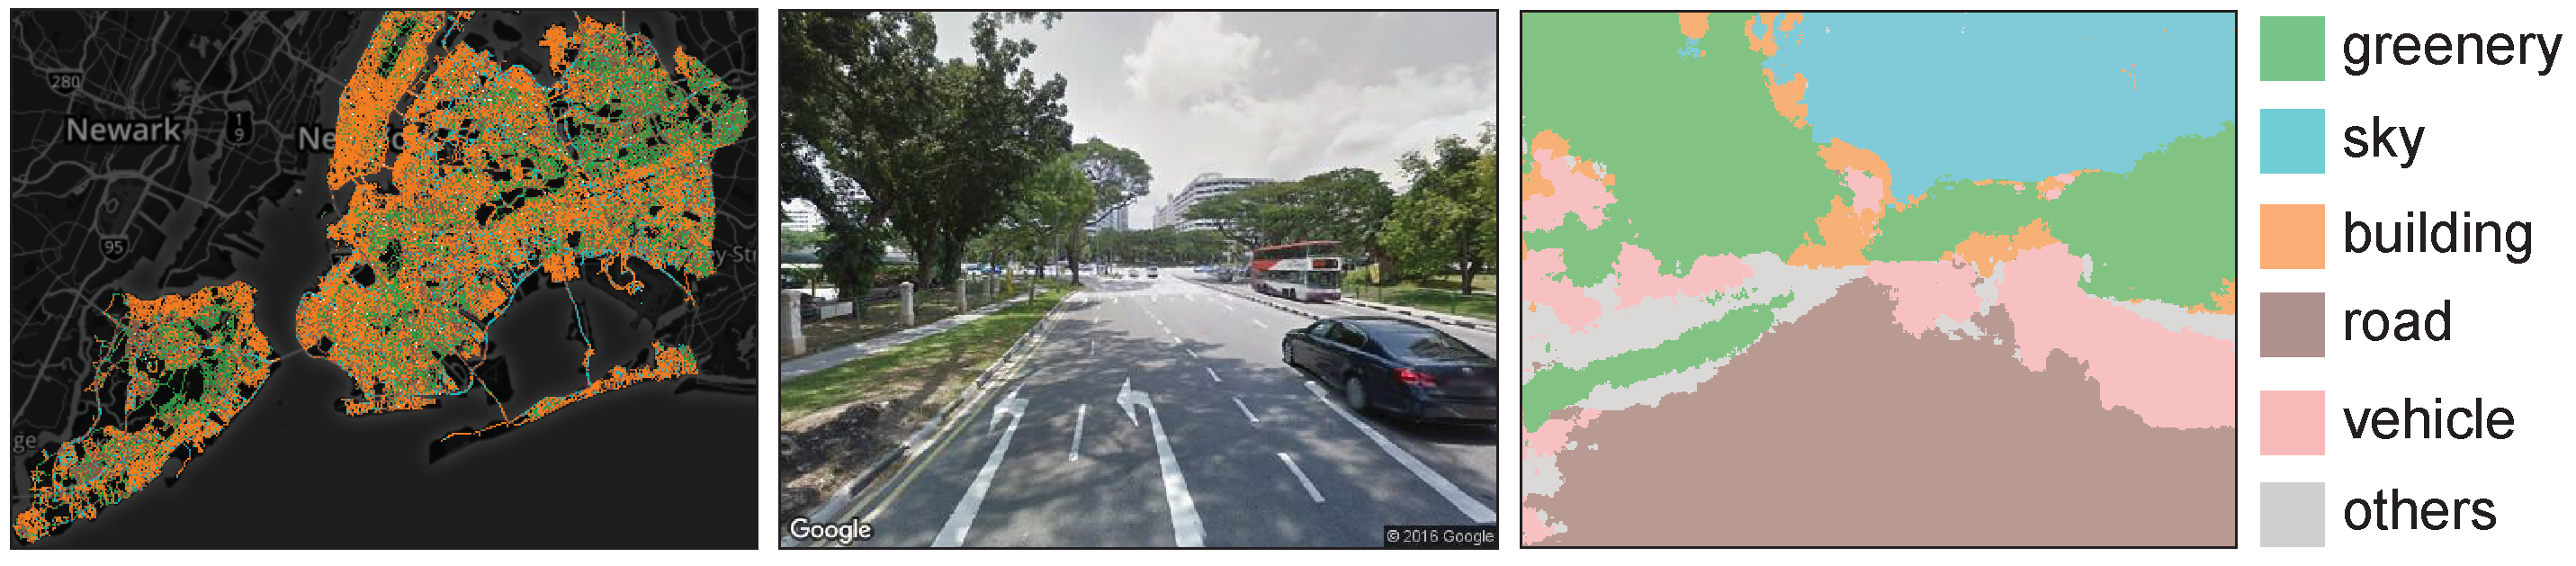
\includegraphics[width=\columnwidth]{figure/streetvizor/fig3_data_preprocess/data_process}
	\vspace{-7mm}
	\caption{Illustration of data preprocessing: sampling locations in New York City are generated from OpenStreetMap (left), a street view image is collected from Google Street View (center), and the image pixels are classified into six features using SegNet (right).}
	\label{fig:c1_data_preprocess}
	\vspace{-1mm}
\end{figure}

%===============================================
\subsection{Data Collection}
\label{ssec:c1_data_collection}

Based on the configurations defined in Section~\ref{sec:c1_bg}, we develop an automatic approach to collect GSV images.
We first download the area of a city from OSM~\cite{osm_api} and extract the road network from the OSM data.
Next, we apply a flood-fill algorithm that recursively goes through the entire road network every 50 meters, starting from a randomly selected location.
After this operation is completed, a list of sampling locations (\{$pos$\}) with geographic information $(lat \; \& \; long)$ is generated.
We then pass each $(lat \; \& \; long)$ into GSV API, and extract the corresponding street information $(SI)$, including street name $(s\_name)$ and heading $(h)$. 
Finally, we download front and back images at each sampling position by passing $lat, \; long \; \& \; h$ with the default field of view and pitch values into GSV API.
Together with the downloaded image ($Img$), we model urban forms at human-scale ($UF_{hs}$) at each sampling location as: 

\vspace*{-5mm}
\begin{equation}
\label{c1_eq_sv}
UF_{hs} \; := \; <pos, \; SI, \; Img>
\end{equation}

We have collected $\sim$147 k, $\sim$183 k, $\sim$685 k and $\sim$637 k images of Hong Kong, Singapore, Greater London and New York City, respectively.
Fig.~\ref{fig:c1_data_preprocess} (left) presents all sampling locations (colored dots) in New York City generated from OSM, and (center) shows a sample street view image downloaded from GSV.

%===============================================
\subsection{Feature Extraction}
\label{ssec:c1_feature}
After collecting street views, we first classify the image pixels into 12 classes (e.g., sky and building) using SegNet~\cite{Badrinarayanan_2015_segnet}, which is a robust pixel-wise semantic labeling tool with a global accuracy of 82.8\%.
Among the 12 classes, we count the number of pixels for the identified five features, i.e., $greenery$, $sky$, $building$, $road$, and $vehicle$, and summarize the remaining pixels as $others$.
We then normalize the feature data because pixel counts ($PC$) as raw output values are not intuitive.
The normalization is straightforward for each feature value ($FV$):
$ FV_i \; = {PC_i} / {PC_{Img}} $, where $i \in \{g, s, b, r, v, o\}$ represent the five features and $others$.
Hence, all feature values are in the range of [0, 1].
Then, we can replace the image ($Img$) with a feature metric ($FM$) as:

\vspace*{-5mm}
\begin{equation}
\label{c1_eq_fm}
Img \rightarrow FM := \; <FV_g, \; FV_s, \; FV_b, \; FV_r, \; FV_v, \; FV_o>
\end{equation}

% The feature extraction is preprocessed on a high-performance workstation with GTX 1080 graphics card. 
% Though enabled with GPU acceleration, the computation still takes from several to up to 20 hours to process the images in each city.
Fig.~\ref{fig:c1_data_preprocess} (right) shows the classification result of the street view image in the center produced by SegNet.

%===============================================
\subsection{Data Querying and Filtering}
\label{ssec:c1_query}

Based on Equations~\ref{c1_eq_sv} and~\ref{c1_eq_fm}, we model human-scale urban forms ($UF_{hs}$) with the following attributes: position ($pos$), street information ($SI$), and feature metric ($FM$).
By nature, the data exhibits the following properties: 
1) $spatial$, i.e., positions;
2) $multi$-$scale$, because the positions can be hierarchically grouped in accordance with city and regional units, or street information;
and 3) $multivariate$, i.e., the feature metric is in six-dimensional data space.

These complex data natures bring in challenges for our analytical tasks.
To address these challenges, we further identify the following querying and filtering models that our system should support:

\vspace*{-2mm}
\begin{itemize}

\item
\textbf{Spatial Query}:
To overview the feature distributions within an AOI (T.1.1), our system should first support an efficient query of a list of \{$UF_{hs}$\} with their $pos$ laying in a given AOI.
The AOI can be either an administrative zone (e.g., a city or a district) or a user-specified region defined using a lasso tool.
We achieve the efficient spatial query operation by organizing all \{$UF_{hs}$\} in a city in a four-level octree structure, in which the topmost level is the boundary of each city.

\vspace*{-2mm}
\item
\textbf{Street Query}:
To support the exploration of human-scale urban forms at street-scale (T.1.2), our system should allow users to interactively query a street by its name.
Here, we create a lookup table with street names as keys, and store corresponding $UF_{hs}$ ids in each street slot.

\vspace*{-2mm}
\item
\textbf{Feature Filtering}:
To accelerate filtering against a particular feature (T.2.2), our system first sorts all \{$UF_{hs}$\} to be explored in increasing order for every feature.
Then, we adopt a binary search approach in run time.

\end{itemize}

%===============================================
\begin{figure}[h]
	\centering
	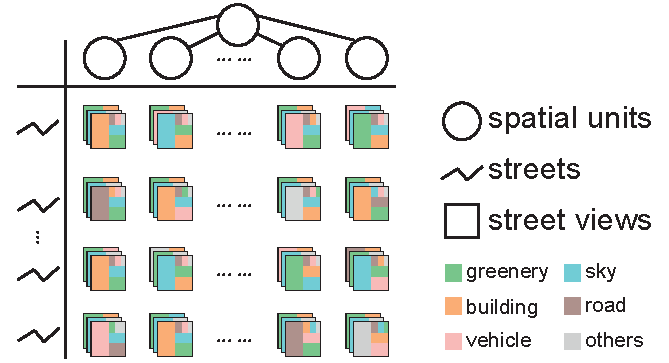
\includegraphics[width=0.8\columnwidth]{figure/streetvizor/fig4_data_model/data_model}
	\vspace{-3mm}
	\caption{Data model: street views with six-dimensional features of \textit{greenery, sky, building, road, vehicle} and \textit{others}, are organized in an octree structure and a street lookup table.}
	\vspace{-1mm}
	\label{fig:c1_data_model}
\end{figure}
\vspace*{-2mm}

Fig.~\ref{fig:c1_data_model} illustrates the data model that organizes the street views in an octree structure and a street lookup table.
Each street view contains the six-dimensional features of \textit{greenery, sky, building, road, vehicle}, and \textit{others}.
We store these querying and filtering models are stored in a back-end MongoDB database, as shown in Fig.~\ref{fig:c1_sys_overview}.
%===============================================

\section{Visualization Design}

In this section, we first discuss the rationales behind our visualization design. 
Then, we provide a detailed description of the visualization techniques implemented in our system.

%============================================================== Teaser

\begin{figure}[t] 
	\centering
	% \vspace{-4mm}
	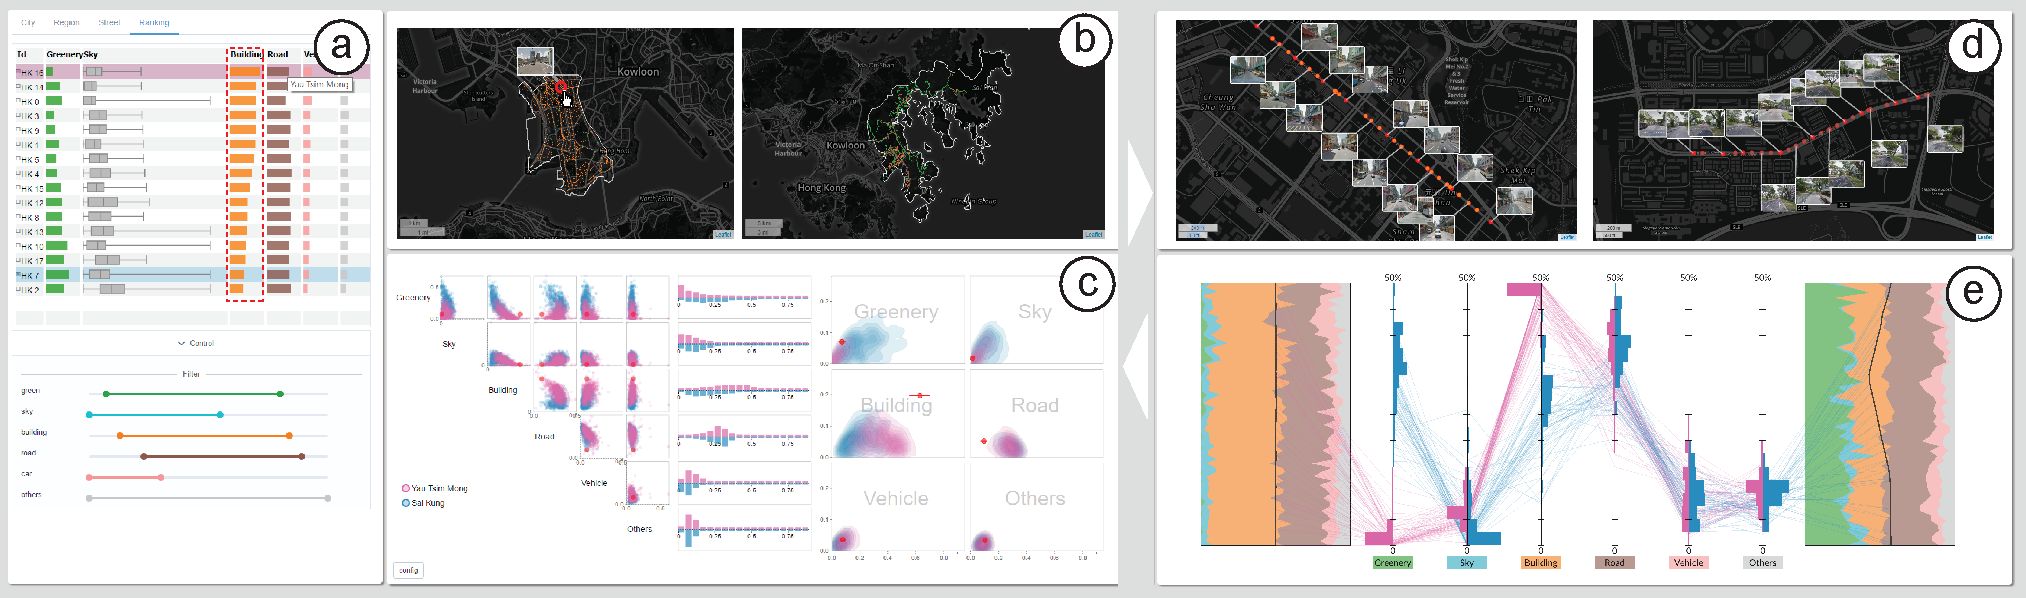
\includegraphics[width=0.9\columnwidth]{figure/streetvizor/fig1_teaser/teaser}
	\vspace{-3mm}
	\caption{StreetVizor system. 
		(a) Control panel enables multi-scale navigation, ranking exploration, and feature filtering.
		(b) Side-by-side map views compare the spatial distribution of human-scale urban forms in two areas-of-interest (AOIs).
		(c) AOI statistic view presents the quantitative measurements, including correlation, histogram, and diversity in the AOIs shown in (b).
		(d) Street map views present detailed street views along two streets.
		(e) Street statistic view extends parallel coordinates with street layouts.}
	\label{fig:c1_teaser}
	\vspace{-5mm}
\end{figure}


%==============================================================

\subsection{Design Rationales}
To address the complex analytical tasks (Section~\ref{ssec:c1_tasks}), a proper visual design should follow the design rationales below:

\begin{enumerate}[label={R.\arabic*:}]

\vspace*{-2mm}
\item
\textbf{Overview+Details}:
To facilitate multi-scale exploration, our system should follow the information-seeking mantra: ``Overview first, zoom and filter, then details on demand"~\cite{shneiderman1996eyes}.
First, the system should provide an overview of human-scale urban forms at city- and region-scales, and then allow users to explore more details at street-scale.
Efficient query and filtering should be provided to enable smooth transitions between these scales.

\vspace*{-2mm}
\item
\textbf{Coordinated Multiple Views}:
Our system should effectively reveal multiple perspectives information of human-scale urban forms, including geographical locations and multivariate features.
CMVs that present linked information and allow users to explore data from multiple joint-perspectives fulfill this requirement.


\vspace*{-2mm}
\item
\textbf{Effective Comparison}:
To enable effective data comparison, different comparative visualization techniques should be employed for multiple-perspective information.
Specifically, given that spatial information for two AOIs/streets is unsuitable for direct overlay, we adopt side-by-side map views.
On the other hand, the feature metric can be mapped on the same scope. 
Therefor, we select a superposition visualization to reveal the differences.

\vspace*{-2mm}
\item
\textbf{Visual Consistency}:
Since multi-scale and multiple-perspective visualizations are to be designed, the system should maintain visual consistency across different visualization modules.
We realize visual consistency by 
1) applying the same layout, i.e., presenting spatial information on the top and quantitative measurements on the bottom, in AOI Explorer and Street Explorer;
2) employing consistent color mappings. 
Specifically, we set green, light blue, orange, brown, light pink, and gray to represent the features of $greenery$, $sky$, $building$, $road$, $vehicle$, and $others$, respectively.
AOIs/streets on the left and right side are colored as red and blue, respectively.

\end{enumerate}

%==============================================================
\subsection{Ranking Explorer}
Ranking Explorer is developed to overview feature attributes across multiple AOI/street candidates to help users quickly identify AOIs/streets for comparison (T.3.1).
The explorer presents each candidate as a row and arranges its multivariate information in seven columns.
The first column provides general information, such as city and region/street id. 
The remaining columns present the six features' mean values as bars, where mean values are normalized and encoded by bar lengths.
Clicking the body of a feature column of interest will expand the column as a boxplot to show statistical distributions.
The explorer also allows users to sort candidates against a particular feature and the ranking will update correspondingly.
Such designs have been well established and evaluated in a previous work~\cite{liu_2017_smartAdP}.

Fig.~\ref{fig:c1_teaser}(a) ranks all districts in Hong Kong in accordance with $building$ feature (red dashed box).
As an example, we observe the detailed statistics of the $sky$ feature.
We select the column for this feature and expand it to boxplot. 
By comparing the orderings of $greenery$, $sky$, and $building$ features, we find $greenery$ and $sky$ features are correlated, while they are negatively correlated with the $building$ feature.
This information helps users narrow down the comparison choices to 1) district HK 16 (Yau Tsim Mong) with the highest $building$ ratio and 2) district HK 7 (Sai Kung) with low $building$ and high $greenery$ ratios, as shown in Figs.~\ref{fig:c1_teaser}(b) \& (c).
% We also find one special region HK 0, which is Central and Western, has both high green feature and building feature. 
% In addition, there is also some street in this region has very high sky feature value. This region could provide a relative good work environment.

% \qm{Even though query methods can effectively help to narrow down to a small scope of AOIs and streets, the planers still need to explore among the small number of candidates. The quantitative ranking and comparison tools based on different features are required for the planers to explore more than two candidates}.
% \qm{The interactions above enable users to narrow down the study scope to several candidates AOIs or streets. To further explore the and find the interested  candidates, we implemented multi-features exploration view (Fig.~\ref{fig:teaser}(a)) which enable quantitative ranking and compare multiple AOIs and streets based on the features interested. Inspired by Lineup~\cite{gratzl2013lineup} and SmartAdp~\cite{liu2017smartadp}, each column indicates one attribute of the AOI/street. The last 6 columns present the six human scale features while other columns present other properties like the id, city they belong to, which can be interactively chosen according to the users' interests. Users can also click on the head to rank the candidates according to the specific features or group several features and rank the candidates by the sum of the selected features.}
%==============================================================
\subsection{AOI Explorer}
\label{ssec:c1_aoi_explorer}
AOI Explorer is developed to provide efficient comparison of human-scale urban forms at city- and region-scales (T.1.1).
The explorer integrates coordinated multiple views, including:

%============================
\subsubsection{AOI Map View}
\label{sssec:c1_aoi_map_view}

We develop side-by-side map views (Figure.~\ref{fig:c1_teaser}(b)) to compare the spatial distributions of human-scale urban forms in two AOIs (T.3.2).
Each map view consists of:
1) a background map layer implemented with Leaflet.js to allow users to change map style (e.g. satellite, street, and sport) for different purposes;
and 2) a point density map overlaid on top of the background map layer, with points representing street views.
The density points are evenly sampled on each street with an upper limit of 10,000 points.
Point color corresponds to the maximum feature value in the street view image.
A corresponding street view image will pop up when the mouse pointer hovers over a point.
Users can select two cities or regions from the navigation panel, or directly manipulate AOIs on the map views with a lasso tool.

Heat map is an alternative design for the point density map.
However, in this work, we focus on the simultaneous analysis of multiple features of human-scale urban forms.
Compositing these features into one heat map~\cite{scheepens_2011_composite} will require redundant user interactions.
In addition, sampling positions are generated along the street network.
Thus, no street views is collected from many places across a city.
In this case, the heat map will generate ambiguity between the two scenarios of 1) no record or 2) low feature values in a region.

\begin{figure}[t]
	\centering
	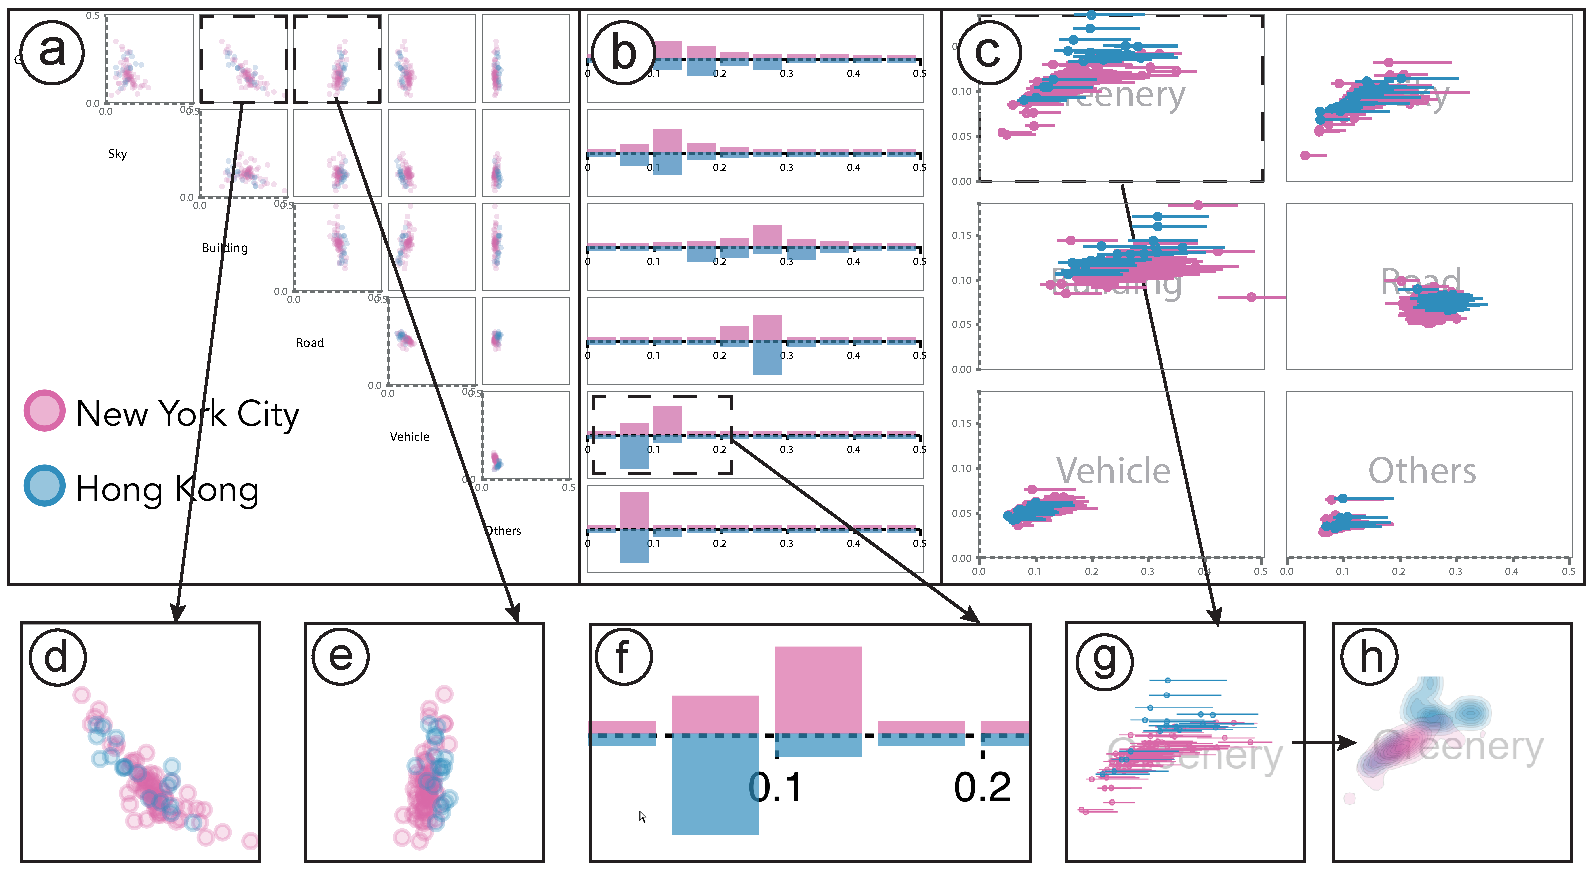
\includegraphics[width=0.85\columnwidth]{figure/streetvizor/fig5_statistic_view/statistic_view}
	\vspace{-4mm}
	\caption{The AOI Statistic View combines (a) a scatterplot matrix to show pair-wise correlations between two features, (b) small multiples of histogram bar charts to overview feature distributions, and (c) small multiples of deviation plots to present feature diversity. }
	\label{fig:c1_statistic_view}
	\vspace{-4mm}
\end{figure}

%============================
\subsubsection{AOI Statistic View}
\label{sssec:c1_statistic_view}
Besides the map view, which enables the comparison of spatial distributions of human-scale urban forms, we develop AOI Statistic View to allow users to compare various quantitative measurements (T.3.3).
Nonetheless, each AOI may contain too many street views (up to several hundred thousand) that will overload the rendering process.
Moreover, the street views will occlude each other if we simply plot all of them.
To address this problem, we cluster street views into groups based on either their administrative units (districts, divisions, and streets) or a mean-shift clustering algorithm~\cite{comaniciu_2002_meanshift} that works as follows.
 
\vspace*{2mm}
\noindent
\textbf{Mean Shift Clustering}.
We cluster urban forms based on their feature metric and geographical positions.
Our algorithm works in the following way: 
given an input list of $N$ human-scale urban forms \{$UF_{hs}$\}, we first normalize the $lat$ \& $long$ attributes of each $UF_{hs}$ against the boundary of all \{$UF_{hs}$\}.
Then, we combine the normalized $lat_{nor}$ \& $long_{nor}$ with the feature metric to construct a new dataset $X := \{x_1, x_2, ..., x_N\}$, where each data point $x_i$ is in an eight-dimensional space, $R^{8} := \; <lat_{nor}, \; long_{nor}, \; FV_g, \; FV_s, \; FV_b, \; FV_r, \; FV_v, \; FV_o>$.
The distance between two data points is measured as their Euclidean distance.
We then estimate a bandwidth $h$ from $X$, and apply mean-shift clustering algorithm on $X$ using a flat kernel.
Here, the bandwidth estimation and mean shift clustering are performed with a machine learning library \textit{scikit-learn}~\cite{scikit-learn}.
Finally, we generate a list of $m$ urban form clusters $C := \{c_1, c_2, ..., c_m\}$, where each cluster $c_i$ contains $n$ data point $c_i := \{x_1, x_2, ..., x_n\}$.

The clustering process groups geographically close street views with similar feature attributes together.
Given that locations are integrated as two-dimensional spaces, the algorithm forms more local clusters than an algorithm without considering spatial information, which usually generates several big clusters with too many street views.
The algorithm may be further improved by adopting a network-based distance measurement approach other than Euclidean distance.
We expect to form more representative clusters of street views with street network information.
Nonetheless, the current approach fulfills our requirement of reducing visual clutter.

\vspace*{2mm}
After generating the clusters $C$, we further compute and visualize the following quantitative measurements:

\vspace*{-2mm}
\begin{itemize}

\item
\textbf{Feature Correlation}:
We first compute the mean values of the identified features, i.e., \textit{greenery, sky, building, road, vehicle}, and \textit{others} in each cluster $c_i$.
We then plot the pair-wise correlations using a scatterplot matrix (Fig.~\ref{fig:c1_statistic_view}(a)).
Notice that the clusters in the left and right AOIs are colored red and blue, respectively.

\vspace*{-1mm}
\item
\textbf{Feature Histogram}:
Though feature values fall in the range of [0\% - 100\%], we seldom find feature values that exceed 50\%.
Thus, we only consider the range [0\% - 50\%].
For each feature, we divide the range into 10 even parts, i.e., [0\% - 5\%), [5\% - 10\%)..., and aggregate the corresponding value in each street view to each part.
Then, histograms for each feature are plotted as bar charts in an up and down manner for AOIs on the left and right, respectively.
The six histogram bar charts are arranged in small multiples next to the scatterplot matrix (Fig.~\ref{fig:c1_statistic_view}(b)).

\vspace*{-1mm}
\item
\textbf{Feature Diversity}:
We use standard deviation to indicate the measured feature diversity measured for each cluster, and design diversity views that are arranged as six side-by-side small multiples for each feature as shown in Figure~\ref{fig:c1_statistic_view}(c).
In every feature diversity view, each cluster is represented as a dot with its x-value indicating the averaged feature value and y-value indicating standard deviation.
In addition, we use line segments to indicate the largest and smallest feature values in each cluster. 
In case an AOI may have hundreds of clusters that lead to serious visual clutter problem, we implement a contour map view~\cite{chen_2014_visual} (Fig.~\ref{fig:c1_statistic_view}(h)) to show overall distribution patterns.
Users can interactively choose one of the views in accordance with different requirements.

\end{itemize}

The AOI Statistic View comparison of New York City (red) and Hong Kong (blue) is shown in Fig.~\ref{fig:c1_statistic_view}.
From the view, we can easily identify some obvious patterns.
For example, in both cities, \textit{greenery} and \textit{building} features are negatively correlated (Fig.~\ref{fig:c1_statistic_view}(d)).
The correlations between other pairwise features, e.g., \textit{greenery} and \textit{road} (Fig.~\ref{fig:c1_statistic_view}(e)), are not obvious.
From Fig.~\ref{fig:c1_statistic_view}(f), we find that the vehicle ratio is higher in New York City than in Hong Kong.
In addition, we find that although the \textit{greenery} values are similar for both cities, diversity is higher in Hong Kong (Fig.~\ref{fig:c1_statistic_view}(g)).
This results reflects that greenery is better integrated into street space in New York City than in Hong Kong.

%==============================================================
\subsection{Street Explorer}
\label{ssec:c1_street_explorer}

\begin{figure}[t] 
	\centering
	% \vspace{-4mm}
	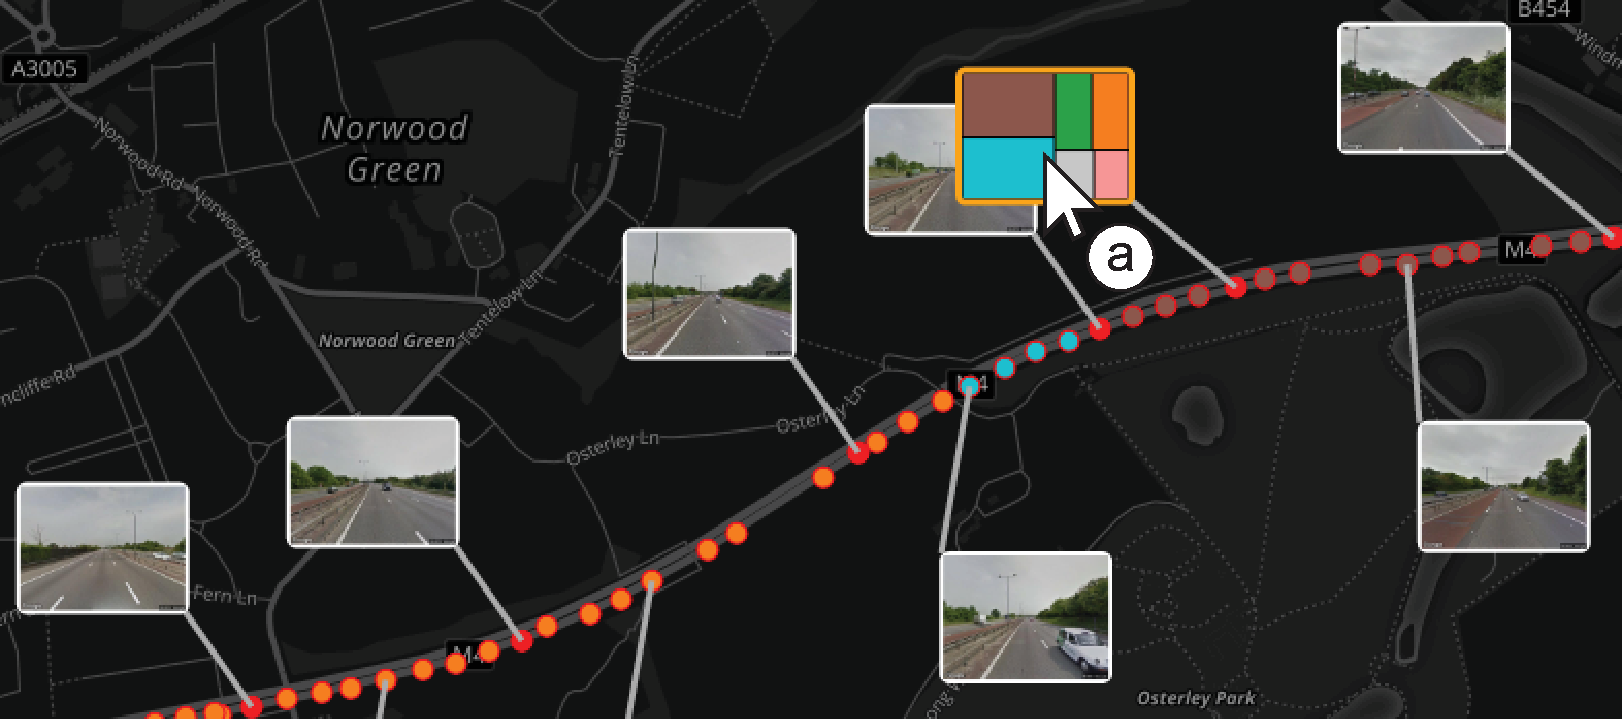
\includegraphics[width=0.9\columnwidth]{figure/streetvizor/fig6_street_map_view/street_map_view}
	\vspace{-3mm}
	\caption{Street Map View provides an overview of all street views along a street as colored points, and highlights images on two sides of the street.
	(a) A tree map showing the feature composition of an image will pop up when the mouse pointer is hovered over the image.}
	\label{fig:c1_street_map}
	\vspace{-5mm}
\end{figure}

%============================

Street Explorer is developed to enable the efficient comparison of human-scale urban forms at street-scale (T.1.2). 
The explorer adapts the same layout as that in the AOI Explorer, i.e., juxtaposition map views are placed on the top of the explorer, whereas detailed statistics view are on the bottom. 

\subsubsection{Street Map View}
\label{sssec:c1_street_view}

Similar to AOI Map View, Street Map View is also developed on top of a background map layer that is implemented using Leaflet.js.
Street views on the street are over-viewed as points with colors that correspond to primary features, i.e., green for $greenery$, light blue for $sky$ and orange for $building$.
In contrast to AOI Map View, Street Map View presents more details of human-scale urban forms by displaying the corresponding street view images along the two sides of a street.
The images are evenly selected in the direction of the street heading. 
In particular, the feature compositions of an image are displayed as a tree map~\cite{shneiderman_1992_tree} when users hover their mouse pointer over the image.
An example is provided in Fig.~\ref{fig:c1_street_map}(a).

%============================

\subsubsection{Street Statistic View}
\label{sssec:c1_street_stat_view}

The design goal for this view is to allow users to quantitatively compare human-scale urban forms from two streets.
Although we can utilize the same views shown in the AOI Statistic View, our collaborating domain expert $SR$ is not satisfied.
$SR$ strongly recommended encoding street layout information in the view, so that users can better leverage their knowledge about streets to perform in-depth analysis.
$SR$ felt the spatial information was not well integrated with the Street Map View.

Based on this goal, we experimented with a few alternative designs and informally evaluated design prototypes with $SR$.
For our first prototype, we designed some glyphs, such as a radial chart or tree map, and directly overlaid the glyphs on the map view.
The design was aborted because isolating statistics on the two maps weakened the effects of comparison.
In addition, such a design easily generated visual clutter, which requires redundant user interactions or clustering to address.
For the second prototype, we encoded street layout information in a similar design as the AOI Statistic View.
However, this method was extremely difficult because the rendering space was fully utilized. 

\begin{figure}[t]
	\centering
	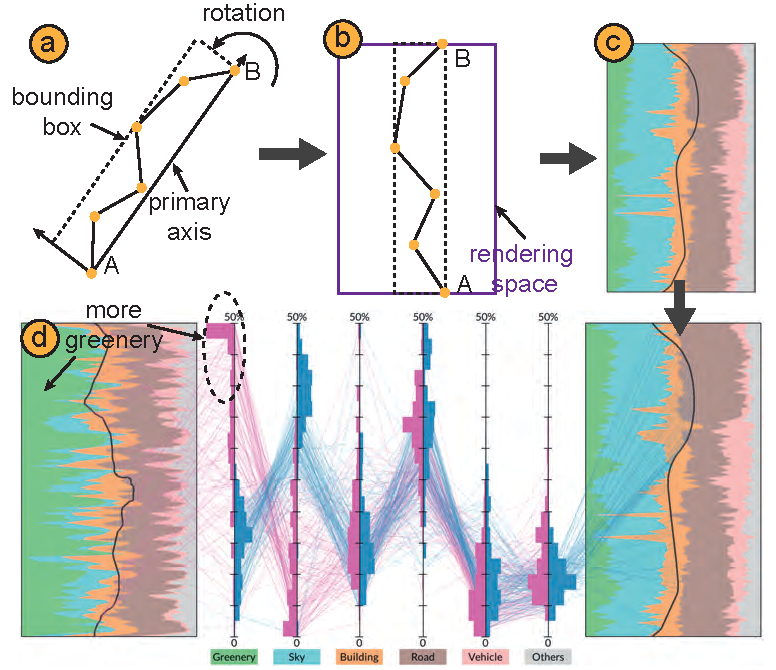
\includegraphics[width=0.9\columnwidth]{figure/streetvizor/fig7_street_model/street_pcp}
	\vspace{-5mm}
	\caption{Overview of the construction process for Street Statistic View:
	(a) Construct minimum bounding box of the street network.
	(b) Rotate the street network such that its bounding box fits in the rendering space.
	(c) Plot themeriver style visualization within the rendering space.
	(d) Enhance parallel coordinates with street layouts on both sides.}
	\label{fig:c1_street_statistic_view}
	\vspace{-6mm}
\end{figure}

\vspace*{2mm}
\noindent
\textbf{PCP with Street Layout}. Inspired by~\cite{qu_2007_visual}, we ultimately develop a design of a parallel coordinates enhanced with street layouts (Fig.~\ref{fig:c1_street_statistic_view}(d)).
We elaborate the construction of this design as follows:

\vspace*{1mm}
\noindent
\textit{Bounding Box Construction} (Fig.~\ref{fig:c1_street_statistic_view}(a)).
The first step is to construct a minimum bounding box ($MBB$) of the street layout.
% , which is represented as lines connecting positions of corresponding street views.
We find the starting ($A$) and ending ($B$) points, and generate a primary axis pointing from $A$ to $B$.
$MBB$ is generated as the minimum rectangle that contains all nodes of the street network parallel with the primary axis.

\vspace*{1mm}
\noindent
\textit{Street Layout Rotation} (Fig.~\ref{fig:c1_street_statistic_view}(b)).
Next, we rotate the street layout such that $MBB$ fits in the rendering space, i.e., $A$ and $B$ lay on the top and bottom (or vice versa) sides of the rendering space, and the rotated $MBB$ lays in the center.
In the case that $MBB$ is wider than the rendering space, the street layout outside the rendering space is clipped.
The rotation direction (clockwise or anticlockwise) is determined based on the direction that produces the minimum rotation angle.

\vspace*{1mm}
\noindent
\textit{ThemeRiver Plotting} (Fig.~\ref{fig:c1_street_statistic_view}(c)).
To fully utilize rendering space, we plot a themeriver-style~\cite{havre_2002_themeriver} visualization to show changes in feature values along a street layout.
Here, the themeriver is plotted in the vertical instead of the traditionally horizontal direction because the street layout is aligned along the y-axis after rotation.
Next, given that street views are sampled evenly along the street layout, we map the street views equally onto the y-axis, i.e., y-values of the themeriver plot reflects the relative positions of street views along the street layout.

We start plotting the themeriver visualization using the left side of the rendering space as the baseline and calculate the upper bound x-values for the $greenery$ feature.
The upper bound x-values of the $greenery$ layer are then used as baseline values for the next feature, i.e., $sky$.
This process is repeated until all features are plotted.
To support better feature comparison, our system allows users to reorder feature sequence by clicking on the feature layer of interest and shifting it to the left side~\cite{byron_2008_stacked}.

\vspace*{1mm}
\noindent
\textit{PCP Integration} (Fig.~\ref{fig:c1_street_statistic_view}(d)).
The themeriver plot can be used as a coordinate for the PCP.
To enable comparison between two streets, we integrate their themeriver plots into a PCP on left and right sides, and the identified features are used as other coordinates.
Each street view is conveniently presented as a polygonal line, which is colored as red and blue for left and right street views, respectively.
In addition, we aggregate the feature values via binning techniques on left and right sides of each feature coordinate to facilitate the visual comparison of feature distributions.

\vspace*{1mm}
Fig.~\ref{fig:c1_street_statistic_view}(d) presents an example Street Statistic View.
A first glimpse at the two themeriver plots, we can find that the left street contains more $greenery$, while on the right street people can see more $sky$.
This can be found in the distribution comparison on the $greenery$ \& $sky$ coordinates in the middle.
Besides, we can also find that feature values vary dramatically on the left themeriver plot, showing street views are very different along the left street.


\begin{figure}[t]
	\centering
	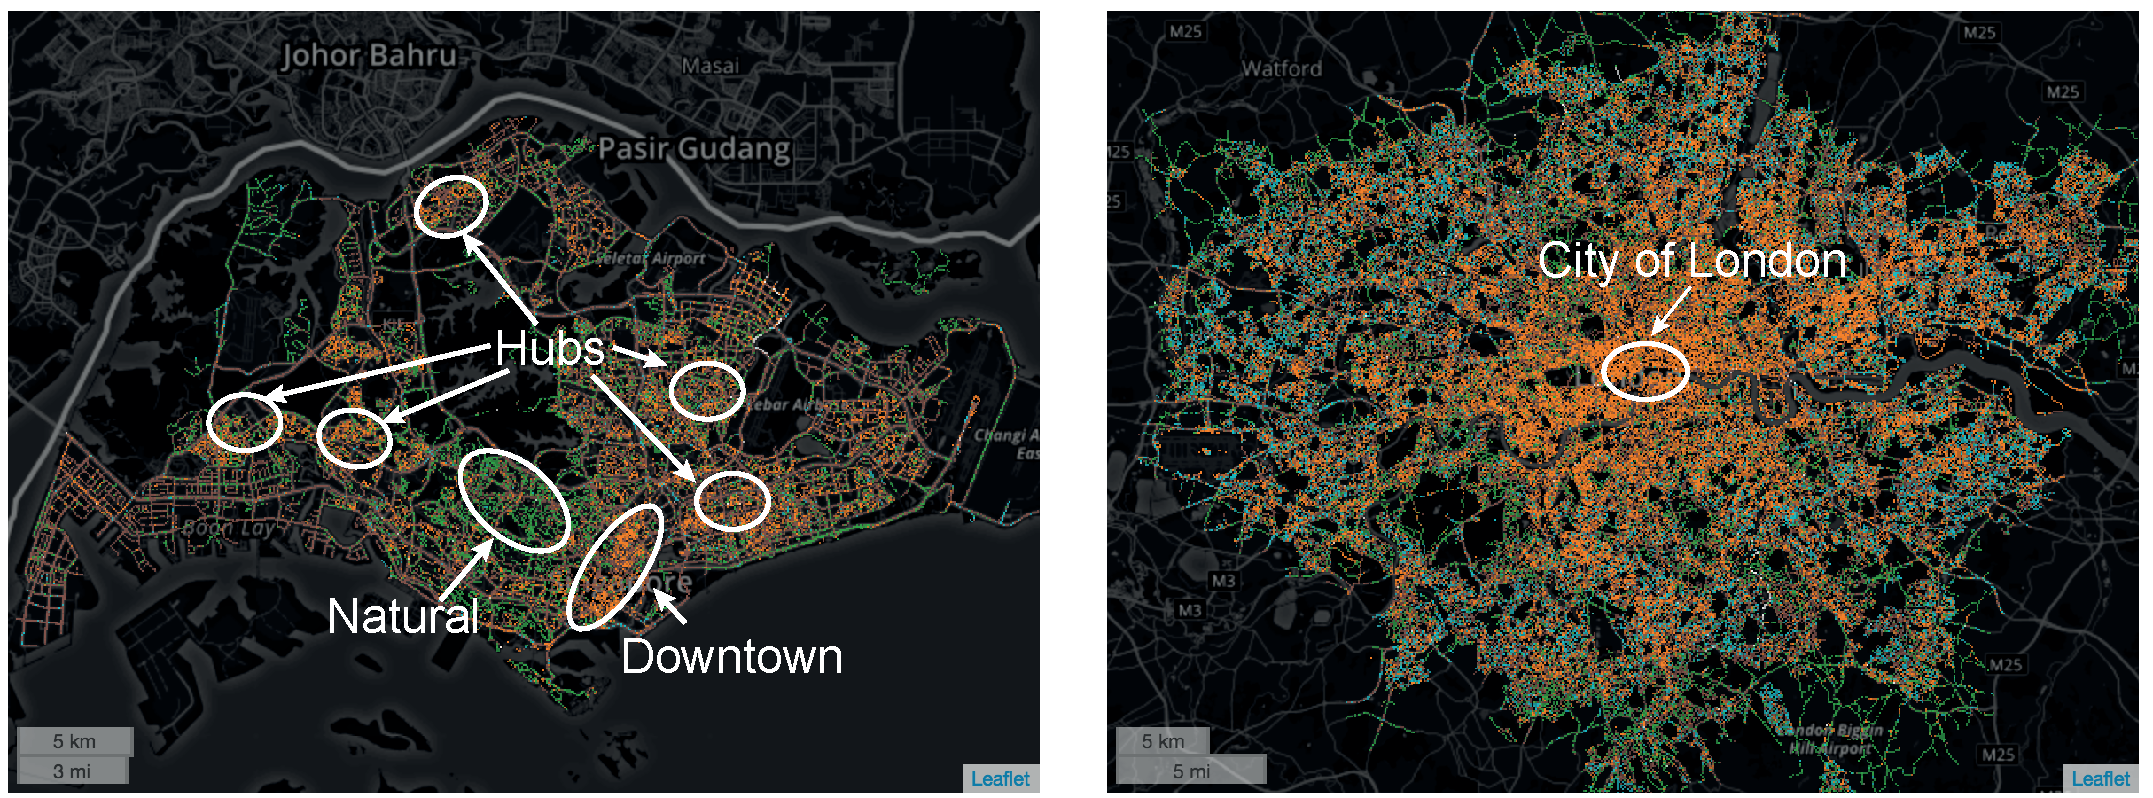
\includegraphics[width=0.95\columnwidth]{figure/streetvizor/fig8_study_1/study_1_spatial}
	\vspace{-4mm}
	\caption{
	AOI Map View compares spatial distributions of human-scale urban forms in Singapore (left) and Greater London (right).
	Orange points (buildings) are concentrated around the highlighted center area of Greater London, i.e., City of London.}
	\label{fig:c1_study_1_spatial}
	% \vspace{-2mm}
\end{figure}

\begin{figure}[t]
	\centering
	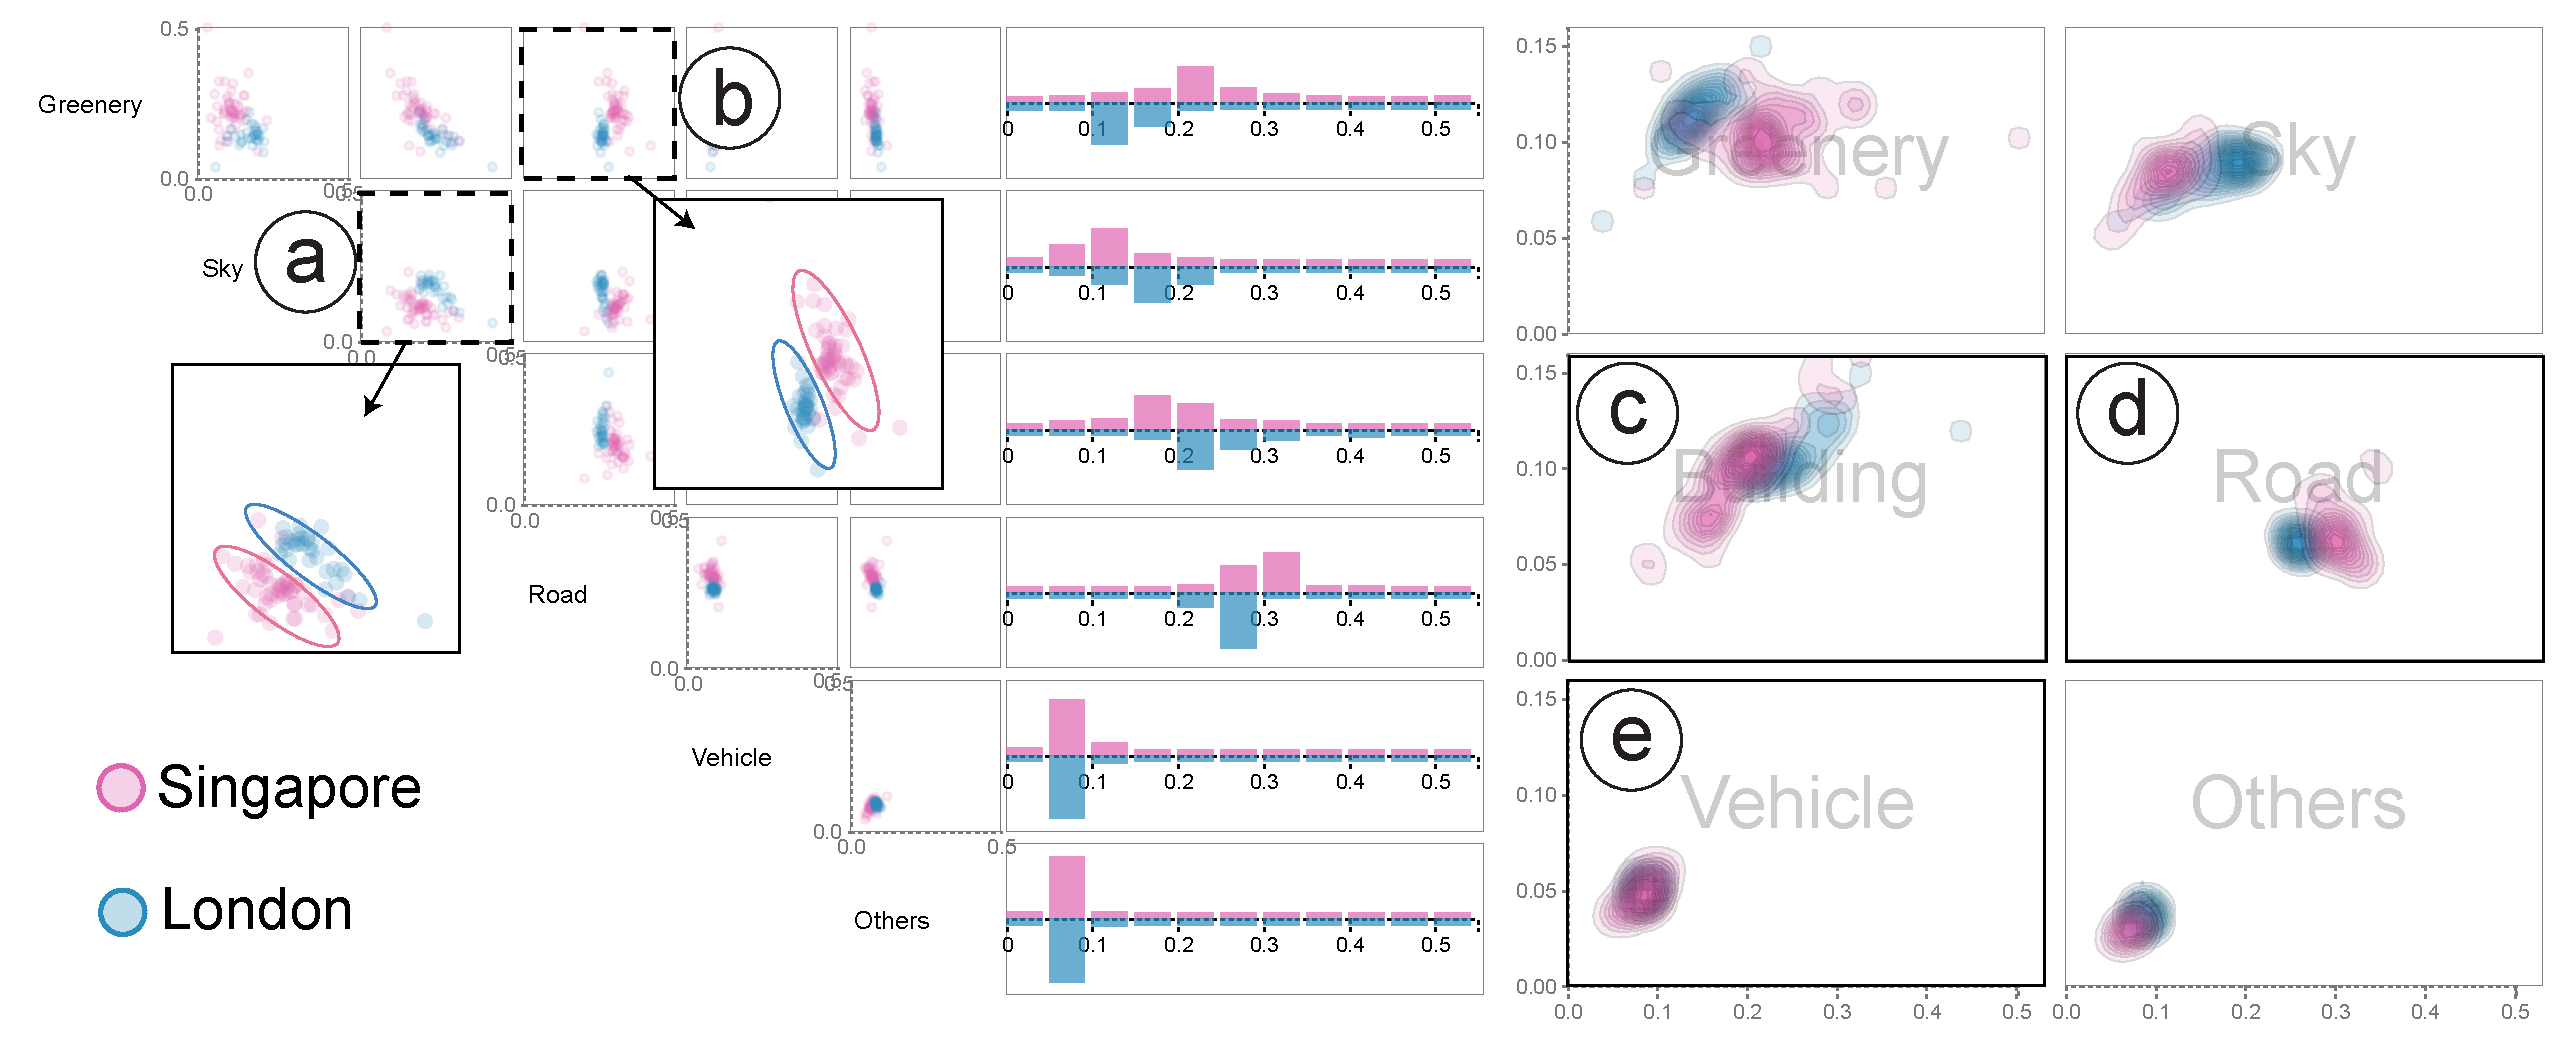
\includegraphics[width=\columnwidth]{figure/streetvizor/fig8_study_1/study_1_statistic}
	\vspace{-7mm}
	\caption{AOI Statistic View in coordination with Fig.~\ref{fig:c1_study_1_spatial} presents quantitative measurements differences of human-scale urban forms in Singapore (red) and Greater London (blue).}
	\label{fig:c1_study_1_statistic}
	\vspace{-5mm}
\end{figure}


%==============================================================
\subsection{User Interactions}
\label{ssec:c1_user_interaction}

\QM{In addition to basic interactions in each view, StreetVizor also provides a control panel (Fig.~\ref{fig:c1_teaser}(a)) that enables:}

\begin{itemize}

\vspace*{-1mm}
\item
\textit{Multi-scale Navigation}.
To help users navigate effectively across different scales, we develop city-, region- and street-panels.
The city-panel lists all four cities, i.e., Hong Kong, Singapore, Greater London, and New York City.
Users start navigation by selecting a city. 
The region-panel will then list all administrative regions under the city.
For instance, City of London and Kingston will be listed if Greater London is selected.
Similarly, the street-panel lists all the streets inside a selected city or region.
% We also provide a region and street query by entering a corresponding name.

\vspace*{-1mm}
\item
\textit{Feature Filtering}.
Our system also supports filtering human-scale urban forms against a specific feature by specifying the value range with feature sliders. 
By default, each feature slide within [0 - 1], and users can change the minimum and maximum values by dragging the slider buttons.

\end{itemize}

In addition, our system also supports the following user interactions to facilitate visual exploration.
\begin{itemize}

\vspace*{-1mm}
\item
\textit{Details on Demand}.
To enable overview+details (R.1), we develop a set of interactions that allow users to explore the details of human-scale urban forms on demand.
For example, if a street view point is selected in the AOI Map View, the corresponding image will show up.
Thus, users can leverage their domain knowledge by visually examining street views.

\vspace*{-1mm}
\item
\textit{Linking}.
Our system supports automatic linking among the visualization modules in both AOI Explorer and Street Explorer for coordination across multiple views (R.2).
For example, if a specific street view on the AOI Map View is selected, the cluster that contains the street view in the scatterplot matrix and the diversity views will be highlighted accordingly.

\end{itemize}
\section{Case Studies}

This section presents three case studies on the application of StreetVizor in assisting urban planners to explore and compare human-scale urban forms on the city-, region-, and street-scales.


\begin{figure}[t]
	\centering
	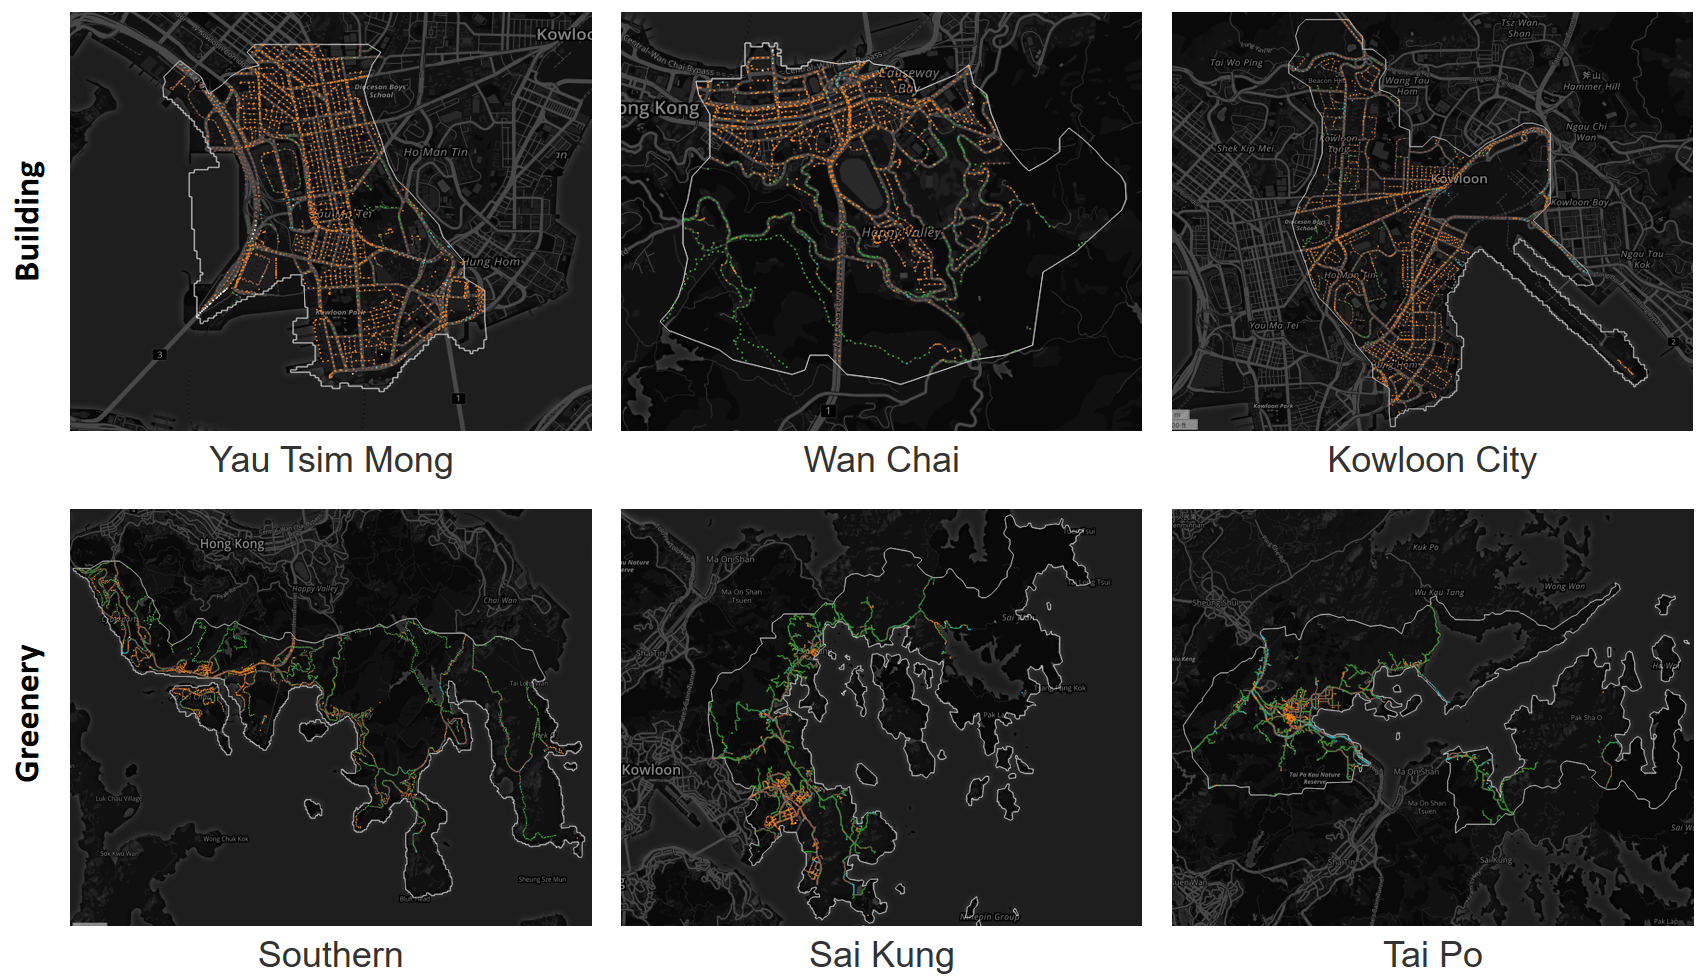
\includegraphics[width=0.98\columnwidth]{fig9_study_2/region-functionality.png}
	\vspace{-5mm}
	\caption{Top three districts with highest $building$ ratios, while bottom three with highest $greenery$ ratios in Hong Kong.}
	\label{fig:region-funcitonality}
	\vspace{-4mm}
\end{figure}

%=================================================
\subsection{City-scale Comparison}

\textit{Comparing Spatial Distribution}.
With the AOI Map View, our system allows users to compare spatial distributions of human-scale urban forms in two AOIs (T.1.1).
Fig.~\ref{fig:study_1_spatial} presents a comparison between Singapore (left) and Greater London (right).
As shown in the figure, more orange points surround the highlighted white circle, whereas more green points can be found at marginal areas in Greater London.
This indicates that more buildings are constructed around the City of London, reflecting that this city is more urbanized compared with other areas.
By contrast, Singapore's urban forms are evenly distributed.
More orange points are found in the highlighted downtown and region hubs, and more green points can be found in natural areas.
Our collaborator $SR$ explained the reason for the different spatial distributions of urban forms in Greater London and Singapore: Greater London likely expanded its urbanization from the City of London to surrounding areas, whereas Singapore, as an island city, cannot expand.
% The reason of this difference between Greater London and Singapore may be that Grater London expands its urbanization from City of London to surrounding areas, while Singapore as an island city cannot expand, as explained by our collaborator $SR$.

\vspace*{2mm}
\noindent
\textit{Comparing Quantitative Measurements}.
We can further explore the differences in quantitative measurements with AOI Statistic View (T.2.1 \& T.3.3).
Fig.~\ref{fig:study_1_statistic} shows the AOI Statistic View in coordination with Fig.~\ref{fig:study_1_spatial}.
From the scatterplot matrix, we find that $greenery$ and $building$ features are negatively correlated.
This result is the same as that shown in Fig.~\ref{fig:statistic_view}(d).
Given that $buildings$ are artifacts and $greenery$ is natural, the negative correlation between $building$ and $greenery$ features in all four cities indicates that artifacts increase and natural environments decrease with increasing urbanization.
To improve livability, many urban planners have proposed integrating more natural spaces in street space.
In addition, Fig.~\ref{fig:study_1_statistic}(a) shows that $sky$ and $building$ ratios are higher in London than in Singapore.
By contrast, $greenery$ and $road$ ratios are higher in Singapore than in London (Fig.~\ref{fig:study_1_statistic}(b)).
These findings can also be found from the middle histogram bar charts.
In addition, the diversity views further show some interesting patterns.
For example, $building$ and $road$ diversities are more concentrated in London than those in Singapore, as shown in Fig.~\ref{fig:study_1_statistic}(c) \& (d), and likely resulted from the different standards for building and road construction in the two cities.
$Vehicle$ usage rates are low in both cities, as shown in Fig.~\ref{fig:study_1_statistic}(e). 


%=================================================
\subsection{Region-scale Exploration}

Given that human-scale urban forms are highly associated with the daily lives of residents, we posit that urban forms could reflect the functionalities of a region.
Study 1 already reveals the negative correlations between $greenery$ and $building$ features, and we hypothesize that these two urban forms can reflect urbanization levels.
To evaluate the hypothesis, we further explore these two features at region-scale (T.1.1).
Using ranking functions, we sort administrative districts in Hong Kong based on these two features.
Fig.~\ref{fig:region-funcitonality} presents an overview of three districts with highest values for each feature. 
The top three districts are Yau Tsim Mong, Wan Chai, and Kowloon City.
They are all business centers in Hong Kong, and we find these districts are mostly covered by orange points ($building$). 
By contrast, the bottom three districts contain highest values for $greenery$.
In particular, the greenest district is Southern Island, which is reserved as country parks.
The other two districts are also well-known natural areas in Hong Kong.
 
\begin{figure}[t]
	\centering
	\includegraphics[width=\columnwidth]{fig9_study_2/study_2_2}
	\vspace{-7mm}
	\caption{Region-scale comparison of Tanglin in Singapore with Central Park in New York City.}
	\label{fig:center-park-tanglin}
	\vspace{-5mm}
\end{figure}

In addition to exploring regions with different functionalities, urban planners are also interested in comparing regions with similar functionalities.
Here, we leverage our knowledge of famous regions in two different cities, i.e., Tanglin in Singapore (see the region highlighted as natural in Fig.~\ref{fig:study_1_spatial}) and Central Park in New York City.
Both of these regions are well-known parks.
After selecting these regions, we find that nearly all streets in the two regions are dominated by green points, indicating that both regions contain considerable $greenery$ as intended.
However, we find some differences between these two regions by looking deeper into the Street Statistics View (Fig.~\ref{fig:center-park-tanglin}).
First, through the feature histogram bar charts, we find that Central Park has slightly higher $greenery$ ratios (A1), whereas Tanglin has slightly higher $building$ ratios (A2).
Though these differences are marginal, they reflect that more buildings are present in Tanglin, partially because Singapore tries to maximize land usage for building construction.
In addition, by grouping street views based on street units, we glean more information from the diversity plots.
Here, we first obtain the overview that $greenery$ feature has relatively higher mean values and deviations than the other five features.
We also find some anomalies.
For example, some streets have relatively low mean values but high deviations for $greenery$ in Central Park (B1), whereas certain streets have high sky visibility in Tanglin (B2), and some streets have very high $building$ ratios in both regions (B3).

The results of this study show that human-scale urban forms are correlated with regional functionalities.
Meanwhile, even though two regions may have the same functionalities, street spaces in regions can be different between two cities.
This may reflect the differences in city planning and development strategies between cities.


%=================================================
\subsection{Street-scale Comparison}
Our collaborating domain expert $SR$ is interested in comparing the fine-grained details of two streets (T.1.2).
StreetVizor meets this requirement with Street Explorer.
Here, we select one street from Brooklyn, New York City, and one from Kowloon, Hong Kong.
Both streets are representative streets of each district.

Fig.~\ref{fig:study_3} presents the visual comparison of these two streets.
The map views provide an overview that nearly half of the street views are mostly green ($greenery$), and the other half are mostly orange ($building$) on the street from Brooklyn.
By contrast, the street views in Kowloon are mostly orange ($building$).
We can observe more details by looking at the street view images.
As shown on the top images, more $greenery$ and $sky$ with low $buildings$ are seen in the left two images, whereas the right two images are filled with $building$ and $road$.
The tree map of the leftmost image shows the street view is well balanced with $greenery$, $road$, $building$, and $vehicle$ features.
Notice that the street view is also highlighted in the bottom Street Statistic View.
More details on the quantitative measurements of street views can be observed in the bottom Street Statistic View.
The themeriver plots clearly show differences in feature distributions:
street views in Brooklyn are more mixed with balanced $greenery$, $sky$, $building$, $road$, and $vehicle$ features, whereas street views in Kowloon are mostly filled with $building$ and $road$ features.
The histogram bars in PCP further confirm this observation: most street views in Kowloon have less than 10\% $greenery$ and $sky$.

Though it is well known in the field of urban planning that New York City is well integrated with natural features and that Hong Kong has more high-rise buildings, $SR$ is excited to see our system can present these differences so intuitively.
``Street Explorer can definitely improve our work efficiency,'' $SR$ commented.


\begin{figure}[t]
	\centering
	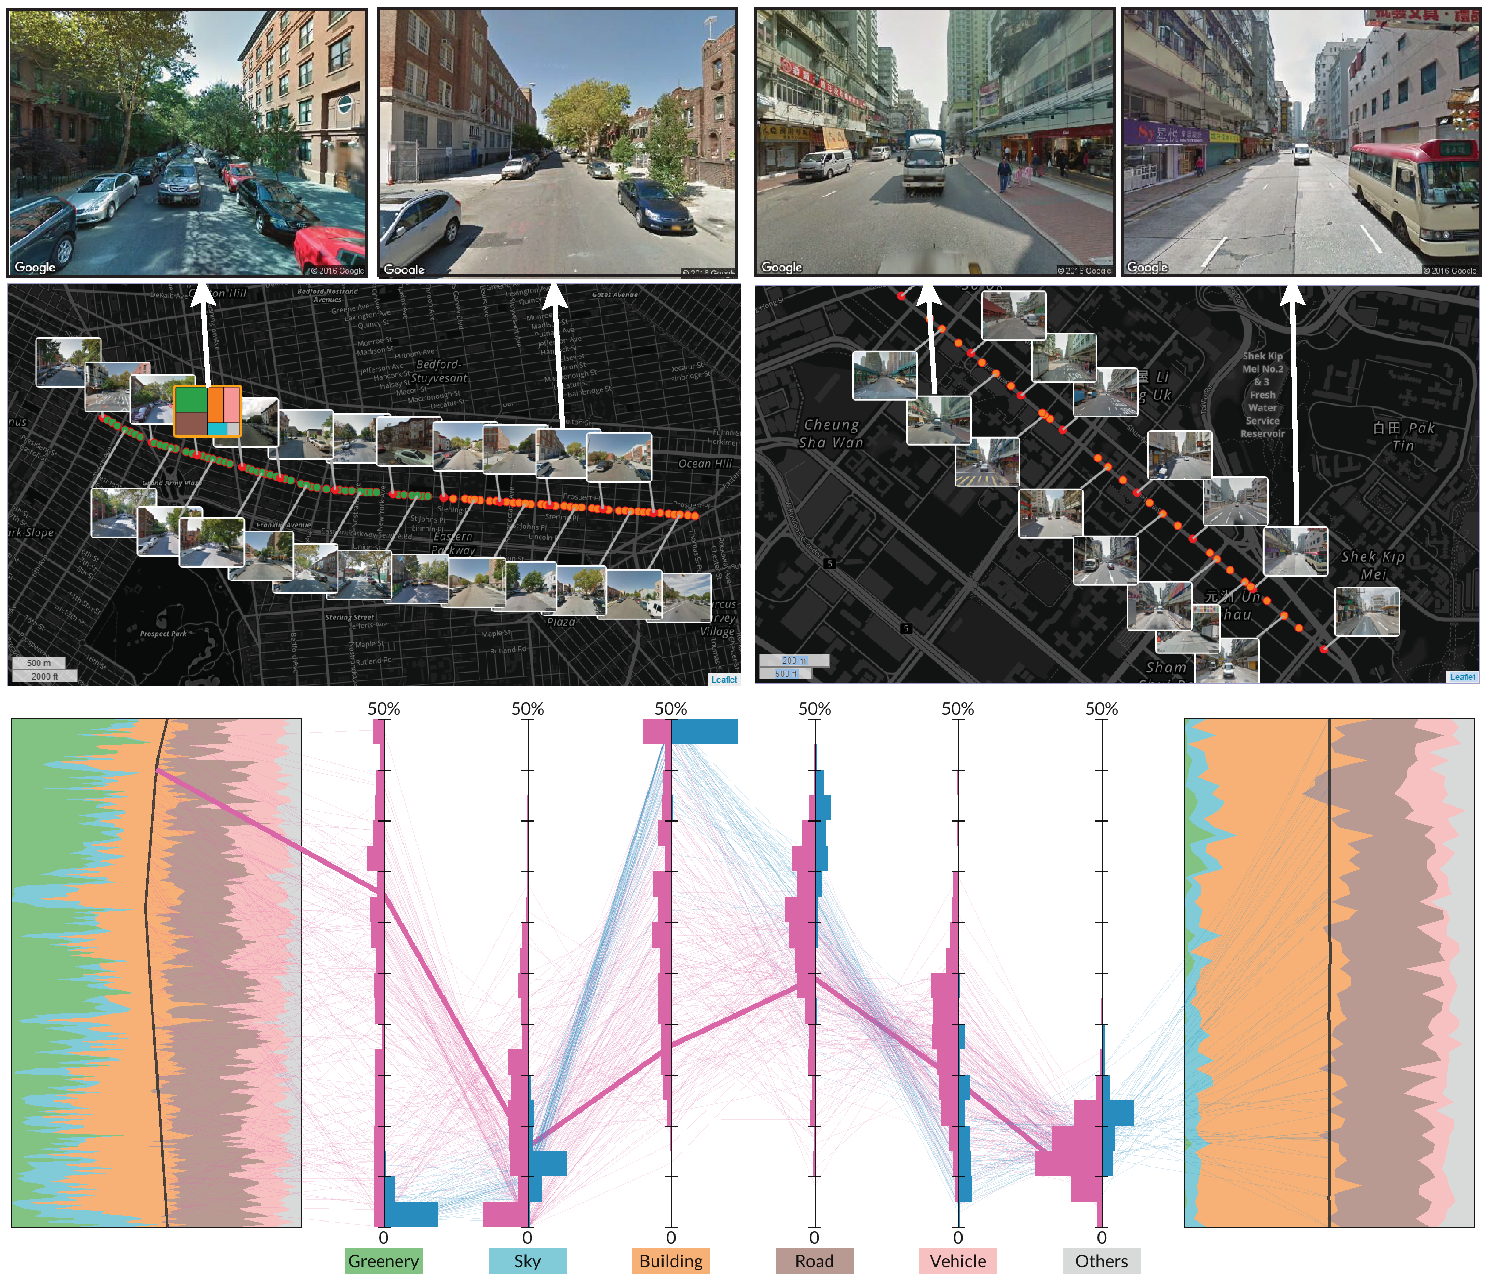
\includegraphics[width=0.95\columnwidth]{fig10_study_3/study_3}
	\vspace{-4mm}
	\caption{Street Explorer compares the differences in human-scale urban forms of two streets in Brooklyn, New York City (left) and Kowloon, Hong Kong (right).
	The left street views contain more balanced features, whereas the right street views are dominated by $building$ and $road$.}
	\label{fig:study_3}
	\vspace{-4mm}
\end{figure}
\section{Expert Review}

To evaluate the effectiveness of StreetVizor, we conducted expert interviews with two independent domain experts other than our collaborating senior researcher $SR$.
One of them focuses on designing livable public space (denoted as $EA$), and the other is an urban ecologist aiming at improving greenery in cities (denoted as $EB$).
Hence, the experts are from different backgrounds: $SR$ and $EA$ in urban planning, while $EB$ in ecology.
In the interviews, we started with explaining the visual encodings and interface design, and demonstrated to them how our system works.
Then, we showed them the case studies, and allowed them to explore the system by themselves for about twenty minutes in the end.
In general, both experts agrees that the way we study human-scale urban forms with street view images is a promising direction.
Their detailed feedbacks are summarized below.

\vspace*{2mm}
\noindent
\textit{Methodology and Approach}.
$EA$ agreed with $SR$ that evidence-based urban design is becoming a trend in urban planning.
He commented, ``StreetVizor is far more than simply a visualization platform. 
Rather, it is an excellent combination of machine learning and visualization techniques, together with classical urban design theories in place-making''.
$EB$ also expressed that ``street view images as an emerging data source can reflect urban environments well", and a visual analytics system can greatly facilitate the exploration of street views.

\vspace*{2mm}
\noindent
\textit{Interactive Visual Design}.
Both experts confirmed that StreetVizor is nicely designed according to the problem domain.
They appreciated the visual consistency across different views.
$EA$ highlighted ``it is very important to use the same colors in different views". 
$SR$ agreed the workflow of ranking multiple AOIs/streets with Ranking Explorer, and comparing two AOIs/streets for details through AOI and Street Explorer is helpful.
``It is easier for me to identify interested regions, such as those in Hong Kong (Fig.~\ref{fig:region-funcitonality})", commented by $SR$.
% They agreed the workflow of over-viewing human-scale urban forms at city- and region-scale first, and examining details at street-scale is helpful.
The AOI Explorer is nicely designed with intuitive map and statistic views.
In particular, ``the statistic view seamlessly integrates three easily understandable plots'', commented by $EB$.
By referring to the scatterplot matrix in Fig.~\ref{fig:statistic_view} \& Fig.~\ref{fig:study_1_statistic}, $EA$ was excited to see the negative correlation between $greenery$ and $building$ $-$ ``there are much space to improve".
$EA$ also liked the visual comparison of human-scale urban form distributions over space (Fig.~\ref{fig:study_1_spatial}), as it reflects the differences of urbanization process and master plans in different cities.

The experts thought presenting street view images in the Street Explorer is intuitive, and mouse hover over to show tree map is helpful.
In contrary, it was difficult in the beginning for both experts to understand the PCP enhanced with street layout information, especially the themeriver plot.
But after exploration, they agreed it is an excellent idea, as it clearly reveals the feature distributions along street.
``Though not common, I believe there are many applications and potentials for the enhanced PCP'', commented by $EB$. 

\vspace*{2mm}
\noindent
\textit{Applicability}.
Both domain experts would like to apply our system to deal with practical problems in their domains. 
Expertized in urban planning and design, $EA$ emphasized ``the lack of efficient tools for human-scale management and design obstacles creating high-quality urban streets.''
 StreetVizor has a great potential to be employed by planners and designers to ``build more pedestrian-oriented and livable streets.'' 
$EA$ also commented ``StreetVizor is highly applicable for evaluating case studies in urban planning''. 
For example, planners can select several key areas, e.g., CBDs, among different cities and then compare their spatial features to develop appropriate strategies in urban renewal.
$EB$ would like to apply our system in environment monitoring, since ``the large amount of GSV images can provide rich information of urban environment''.
He suggested to extend our system in exploring a time-series street view dataset, so that it would allow him to monitor environment changes.

\vspace*{2mm}
\noindent
\textit{Limitations and Improvements}.
The experts pointed out some limitations in our system.
In this work, we explore only six features of human-scale urban forms.
Both experts suggested to extract more urban forms, such as aesthetic amenities and mental well-being, from street view images.
This will advance our system's analytical capabilities and extend its applicabilities.
For instance, a recent study~\cite{jiang_2014_dose} shows that certain relationship may exist between street greenery \& sky ratio and the risk of health challenges.
Besides, they proposed to improve our visual designs.
$EB$ noticed the feature histogram bars in AOI and Street Statistic View are designed differently: one in horizontal, and the other one in vertical style.
He felt the vertical histogram bars are confusing, as they ``do not fit our work habits''.
$EA$ suggested the Street Statistic View can be further improved, by ``encoding neighboring street layouts in the plot'', to reflect spatial information better.

\section{Discussion}
\label{sec:c1_discussion}

In this work, we combine automatic machine learning and interactive visual analytics techniques to explore human-scale urban forms.
The combination of methods tackles the challenges of integrating information from multiple perspectives and at different scales for analysis.
This approach is attractive for urban planners~\cite{liu_2015_understanding, long_2017_how} because it shows the possibility of transferring traditional subjective and intuitive-oriented urban design to evidence-based and big-data informed methods.
%The case studies show that our approach effectively assist domain experts in finding the street view patterns of interest.

The analysis of human-scale urban form in this work relies heavily on a deep learning technique for image classification.
Therefore, classification accuracy poses serious challenges in our approach.
We select SegNet, which achieves a global accuracy of 82.8\%, out of the different classification techniques that we tried.
The case studies show that the classification technique could provide reasonable analytical results on city- and region-scale human-scale urban form patterns.
Nonetheless, the results remain unsatisfactory in many cases, especially when users would like to examine fine detailed urban forms at street-scale.
We envision applying a more advanced classification algorithm in the near future, given the rapid evolution of image classification techniques.
In addition, the classification is preprocessed offline.
Our system does not support the analysis of street views queried on runtime. 
Thus, its applicability is limited and domain knowledge of planners are underutilized in exploring street views in other cities.
This deficiency can also be resolved with advancement in image classification algorithms and machine computing capabilities.

Moreover, we expect that our system will face scalability issues when the number of street view images increase (e.g. when analyzing street views in more cities). 
To tackle this problem, we can integrate more advanced data structures, such as nanocubes~\cite{lins_2013_nanocubes} or Gaussian cubes~\cite{wang_2017_gaussian} for spatial data querying.
More levels of detail and abstraction can also be introduced to handle this problem.
The increase in image number will also burden street view clustering in the interactive exploration process.
We anticipate that certain pre-configurations will facilitate this process.

Presenting multivariate data with spatial information is challenging.
We tackle this challenge by integrating popular PCP with a themeriver plot along an adjusted street layout.
The case studies and feedbacks from experts demonstrate the effectiveness of this design.
Nonetheless, there are some issues with our design.
First, it represents street layout as a simple spline, which is not sufficiently intuitive when the street is straight.
We plan to encode more semantic labels, such as neighboring streets, in the design, as suggested by $EA$.
Second, although the majority of the streets (over 95\%) that we have explored can be rotated and fitted in the rendering space, adjustment does not work in some cases.
Typical examples are streets in a spiral layout.
A more general approach should be developed that can reveal the street layout intuitively and seamlessly fit the street layout in the rendering space.

\input{chapter/2_StreetVizor/10_Conclusion}
